
% EPL master thesis cover template
\documentclass{eplmastersthesis}

\usepackage{todonotes}
\usepackage{hyperref}
\usepackage{subcaption}
\usepackage{bookmark}
\usepackage{tabularx}
\usepackage{listings}
\usepackage[]{algorithm2e}
\usepackage[acronym, toc]{glossaries}


% Fill in here the information: title, student name, speciality, jury members
\title{Network Administration Tool For the Internet of Things}	% Master thesis title
% \subtitle{Subtitle (optional)}			% Optional subtitle
\author{Eddy \textsc{Ndizera}}	% Student name
\secondauthor{Ivan \textsc{Ahad}}	% Second student name if applicable
\speciality{Computer Science}		% Speciality (use one of the following options):
										% Biomedical Engineering
										% Chemical and Materials Engineering
										% Civil Engineering
										% Computer Science
										% Computer Science and Engineering
										% Electrical Engineering
										% Electro-mechanical Engineering
										% Mathematical Engineering
										% Mechanical Engineering
										% Physical Engineering
%\options{Option(s)}		% If required by program commission mention options
\supervisor{Ramin \textsc{Sadre}}	% 1st supervisor name
%\cosupervisor{Firstname \textsc{Lastname}}	% 2nd supervisor name if applicable
\readerone{Olivier \textsc{Bonaventure}}		% 1st reader name
\readertwo{Lionel \textsc{Metongnon}}		% 2nd reader name
%\readerthree{Firstname \textsc{Lastname}}	% 3rd reader name
\years{2016-2017}	% Academic year

\makeglossaries
\newacronym{iot}{IoT}{Internet of Things}
\newacronym{wsn}{WSN}{Wireless Sensor Networks}
\newacronym{gui}{GUI}{Graphical User Interface}
\newacronym{ipfix}{IPFIX}{IP Flow Information Export}
\newacronym{html}{HTML}{HyperText Markup Language}
\newacronym{css}{CSS}{Cascading Style Sheets}
\newacronym{rfid}{RFID}{Radio-Frequency Identification}
\newacronym{ietf}{IETF}{Internet Engineering Task Force}
\newacronym{6lowpan}{6LoWPAN}{IPv6 over Low power Wireless Personal Area Networks}
\newacronym{rpl}{RPL}{Routing Protocol for Low-Power and Lossy Networks}
\newacronym{coap}{COAP}{Constrained Application Protocol}
\newacronym{iana}{IANA}{Internet Assigned Numbers Authority}
\newacronym{rest}{REST}{Representational State Transfer}
\newacronym{json}{JSON}{Javascript Object Notation}
\newacronym{mj}{mJ}{millijoule}
\newacronym{mah}{mAh}{milliampere hour}
\newacronym{mw}{mW}{milliwatt}
\newacronym{mqtt}{MQTT}{Message Queue Telemetry Transport}


\begin{document}

\maketitle					% To create front cover page
\thispagestyle{empty}		% To suppress header and footer on the back of the cover page

\section*{Acknowledgements}

\listoftodos

\tableofcontents
\newpage

\printglossary[type=\acronymtype,nonumberlist]
\listoffigures
\listoftables

\section{Introduction}

-Talk about how predominent is Iot nowadays.
-Talk about how there is no internal monitoring tool for IoT.
-Talk about different sections of the thesis.


\part{State of the art} \label{part:state_art}

\chapter{What is the Internet of Things?}

The Internet of Things or IoT, also called Internet of Everything, Web of Things, can be viewed as the interconnection of things, often referred as objects, motes or smart objects. The Global Standards Initiative on Internet of Things (IoT-GSI) defined \textit{Internet of Things} as "\textit{a global infrastructure for the information society, enabling advanced services by interconnecting (physical and virtual) things based on existing and evolving interoperable information and communication technologies}" \cite{ituitu}. They also give an explanation about what they consider a \textit{"thing"} to be. A thing is "\textit{an object of the physical world (physical things) or the information world (virtual things), that is capable of being identified and integrated into communication networks}" \cite{ituitu}. Fig.\ref{fig:iot} depicts the Internet of Things.\\

\todo[inline]{Give other examples as industry automation or smart cities, or healthcare. (see architecting iot article)}
With the IoT, we dispose of networks constituted by devices which have the ability to communicate between them to exchange data. Also those devices can interact with their environment with means of sensors or actuators. An illustration of such network would be the \textit{Smart Home}. With Smart Home, automation comes into our house. The idea is to have, for example, your door talking to the lights to tell them to light on or to light off depending on if you enter or leave the room. You could have that your alarm would tell the coffee machine to prepare some coffee when ringing in the morning or that your thermostat would regulate the heat of the house. Also, you could remotely manage your house by activating or deactivating the heat and so on. While discussing the presence of the IoT in homes, one field that could largely benefit from the IoT is the field of \textit{e-health}, thanks to the medical monitoring of elderly, ill, and disabled patients, while they would still be in their house and keep their autonomy in their daily life. Smart objects could either be implanted in or around the patient, and information is retrieved from their situation to have regular checkups on their condition(s). The information is then sent and analyzed by specialized staff, ready to intervene if needed. The advantage here is having the ability to remotely monitor patients' situation. (source : architecting the iot).\\

\begin{figure}
  \centering
  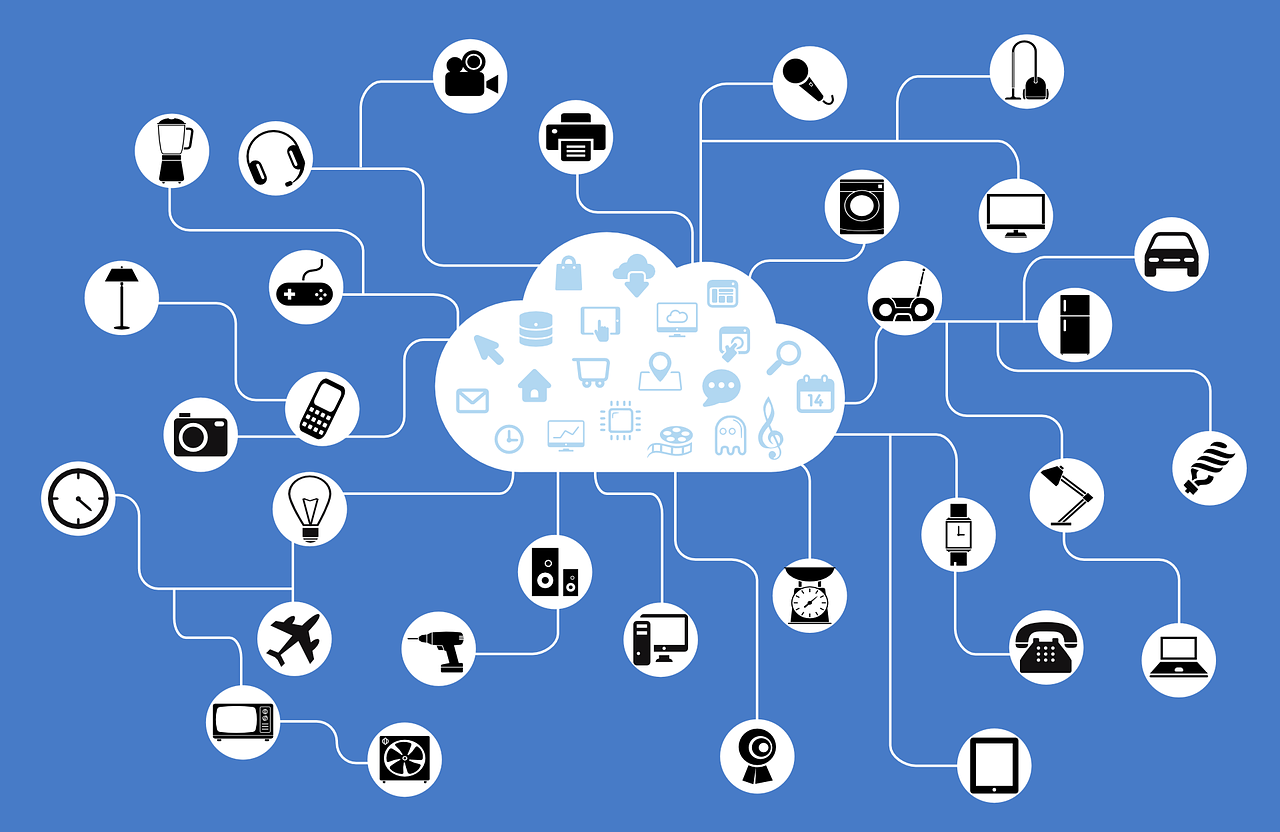
\includegraphics[width=\textwidth]{res/iot.png}
  \caption{Internet of Things (Source: \url{pixabay.com})}
  \label{fig:iot}
\end{figure}

But IoT is not limited only to home. It is already deployed on organizations. For example, the start-up Epicenter injects microchips into their employees (after agreement)\cite{website:lat_04_17}. The microchip enable an employee to open a door or to operate a printer by just a wave of the hand. Also it permits to track them inside the building and permits a colleague to know your whereabouts. \\

The Internet of Things can also be used in many more situations. Power grids can now be better controlled and managed with smart objects, the temperature in buildings and houses can now be monitored and smart objects control radiators and air conditioners to modify ambient temperature, and thus make a more efficient consumption of energy. Shipping containers could also be equipped with devices to better help monitor and modify the climate inside, thus making sure food, clothing, and various materials are better taken care of. Environments hard to analyse like glacier or mountains becomes easier to monitor as we only need to place sensors nodes that will periodically send us the data retrieved from the environment such as temperature. \\

\todo[inline]{Speak about \textit{Industrial Revolution} and \textit{Industry 4.0}}

Those examples show how much we could benefit from IoT. It could improve our efficiency in term of energy but also in term of production. But also could make our life easier by automating certain aspects of the life. In the following subsections, we will go deeper into some technical aspects of the Internet of Things. \\

\todo[inline]{Challenges of iot : preface of book (page xx) + slide 17 du premier cours de mobile.}


\section{Smart Objects}

Smart objects are the main components of an IoT Network. We will explain what makes them special and the purpose of their use.\\

Smart objects, also called IoT Devices, smart devices or connected devices, are physical objects, that are embedded with an electronical component, that allows them to communicate with other objects. Those objects are composed of a software, are equipped with a microprocessor, a sensor or an actuator that allows them to interact with the physical environment and modify/control it, and network connectivity to allow exchange and collection of data. Thanks to network connectivity, devices can sense and exchange sense data of the physical world with each other. They are also often equipped with a small battery, that provides a power source to the device. The connectivity is assured by wireless in most cases. Fig.\ref{fig:smart_objects} shows examples of smart objects.\\

\begin{figure}
    \centering
    \begin{subfigure}[b]{0.3\textwidth}
        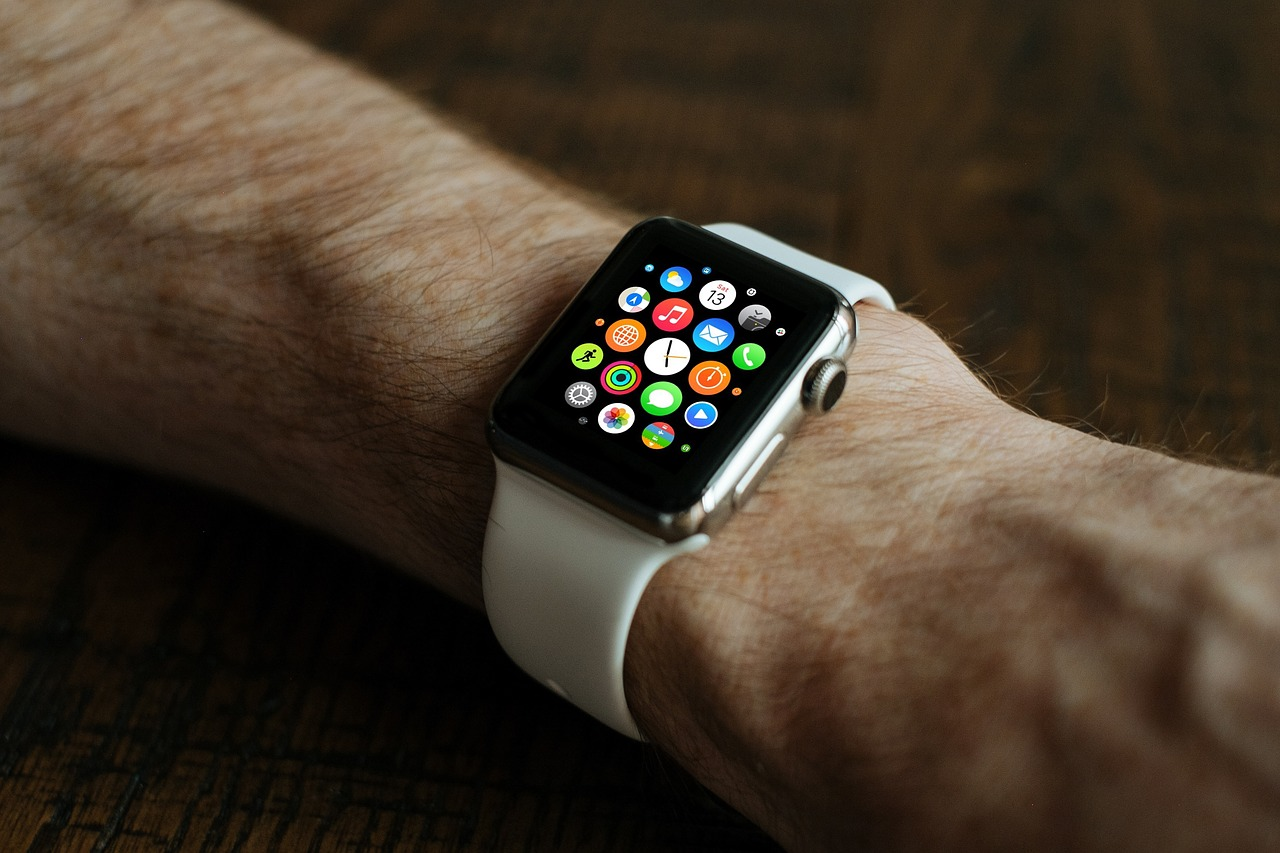
\includegraphics[width=\textwidth]{res/smart_watch}
        \caption{A smart watch}
        \label{fig:smart_watch}
    \end{subfigure}
    ~
    \begin{subfigure}[b]{0.3\textwidth}
        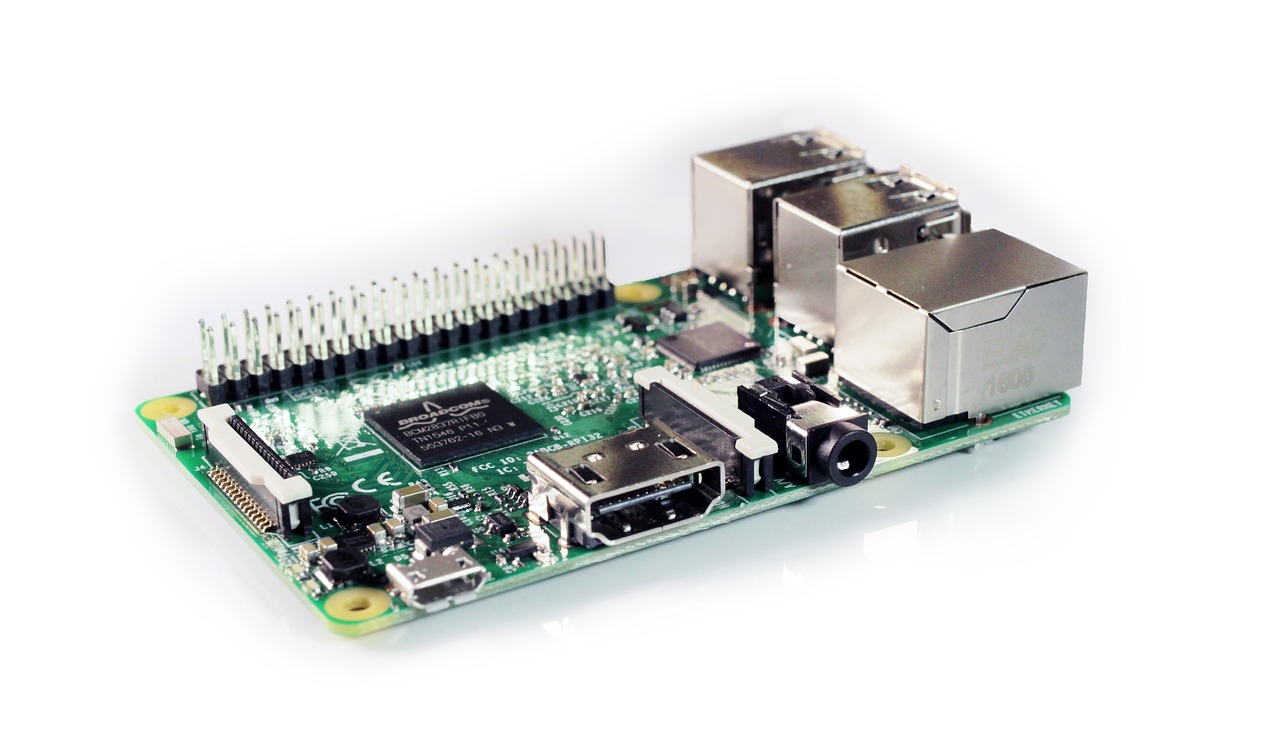
\includegraphics[width=\textwidth]{res/raspberry_pi}
        \caption{A raspberry pi}
        \label{fig:raspberry}
    \end{subfigure}
    \caption{Smart objects (Source: \url{pixabay.com})}\label{fig:smart_objects}
\end{figure}

While it seems pretty straightforward, there does not seem to be a fine line of what exactly smart objects refer to. They may refer to the actual small device with processing and interacting capacity, or the bigger entity that is a physical object made "smart" by the addition of a sensor or actuator. In our case we will consider the latter definition of what an IoT device is. Also in this thesis, we will often employ the terms motes, nodes, devices, smart objects or things interchangeably. \\

Those devices are quite limited also in term of resources. Those are small embedded devices with low power cpu and a limited memory size. Also they are not plugged meaning they rely mainly on their battery. To maximize the battery lifetime, they often switch between awake phases, where the mote is able to communicate and execute process, and sleep phases, where the mote does nothing. Additionally, their wireless range do not permit them to often communicate directly with all members of the network. This is why most of the IoT networks are organized in a hop-by-hop fashion. \\

Tab.\ref{tab:sensors_char} gives some component characteristics about some devices. The raspberry pi 3 presents good specifications. This is typically the type of device that would be used as sink node or data aggregator or data analyser inside an IoT network. The other devices, the MTM-CM5000-MSP and Zolertia Firefly, are mainly sensor motes. They are used to sense the environment and transmit the values. They are not intended for intensive applications. They do not need high specifications and this is why they present low characteristics compare to the Raspberry. But when designing protocols for the Internet of Things, this is those low power devices that must be taken into account as they are the most restraining. \\

\begin{table}
  \centering
  \begin{tabularx}{\textwidth}{|X|X|X|X|}
    \hline
    Model & MTM-CM5000-MSP & Zolertia Firefly & Raspberry pi 3 \\ \hline
    CPU & 8MHz MSP430 & 32MHz ARM Cortex-M3 & 1.2GHz 64-bit quad-core ARMv8 CPU\\ \hline
    RAM & 10KB & 32KB & 1 GB \\ \hline
    Wireless & IEEE 802.15.4 2.4GHz Wireless Module (up to 250Kbps) & IEEE 802.15.4 2.4GHz Wireless Module (up to 250Kbps) & 802.11n Wireless LAN (up to 600Mbps)\\ \hline
    Dimension & 84.4x36.25x13.30mm & 68x25mm & 85 x 56 x 17 mm \\ \hline
  \end{tabularx}
  \caption{IoT devices characteristics}
  \label{tab:sensors_char}

\end{table}

As \cite{chui2010internet} states, the main purpose of smart objects is automation, to replace human intervention for specific computations and data collection. Obviously, they allow the \textit{collection} of bigger loads of data at a faster pace. Once data is collected, the next step is to make actual conclusions about data information. From that point, according to those computations, instructions are passed through the IoT network and the network can enter the process of modifying the physical world through actuators, in an automated fashion and again with no human intervention once the IoT network is set up.\\

To go along with automation, the Internet of Things aims at \textit{optimizing} how it affects the physical world, in terms of energy consumption efficiency, timing, accuracy, etc.

\section{Network Organization}

An IoT network can serve different purposes leading to different topologies. Three topologies are worth to mention as seen in \cite{website:3topo}. Those are:
\begin{itemize}
  \item \textit{Point-to-Point} where a direct connection is configured between two points. An example would be a bluetooth pairing between a laptop and a hi-fi station. It is not widely deployed in industrial IoT as the network cannot scale outside of the two nodes.
  \item \textit{Star} (see Fig.\ref{fig:star}) topology where all nodes communicate via a central hub. All the nodes dispose of a direct link to the central hub. This topology of network is easy to analyze as all traffic must pass through the central hub. However the major disadvantage of it is that the network is limited to the range of communication of the weakest node.
  \item \textit{Mesh} (see Fig.\ref{fig:mesh}) networks are composed of three types of nodes. First, we have simple sensors nodes that only transmit their data. Then we have sensor/router nodes that act as simple sensors nodes but must act as relay for packets of other nodes. Finally, the gateway node that is the intermediary between the network and Internet. This topology is characterized by a communication done in hop-by-hop fashion. It is quite difficult to analyze as we do not know in advance how the routing will be done. Still, the big advantage is the wide surface that the network can occupy and the resiliency due to the number of paths available.\\
\end{itemize}

\begin{figure}
    \centering
    \begin{subfigure}[b]{0.3\textwidth}
      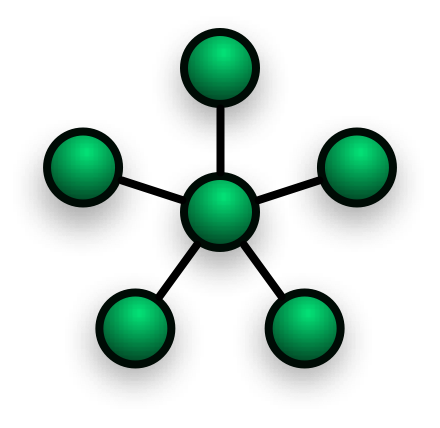
\includegraphics[width=\textwidth]{res/star.png}
      \caption{Star topology}
      \label{fig:star}
    \end{subfigure}
    ~
    \begin{subfigure}[b]{0.3\textwidth}
        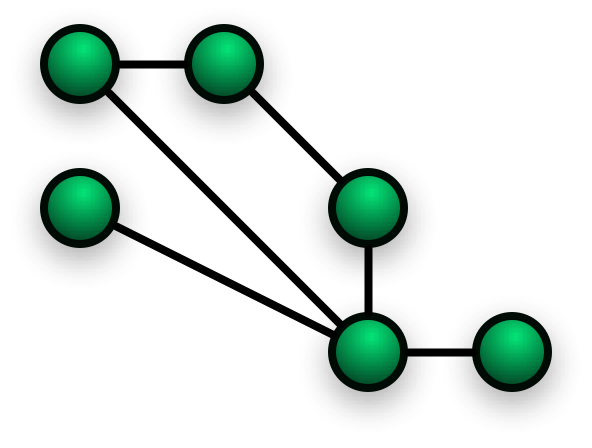
\includegraphics[width=\textwidth]{res/mesh.png}
        \caption{Mesh topology}
        \label{fig:mesh}
    \end{subfigure}
    \caption{Network topologies (Source: \url{en.wikipedia.org/wiki/Network_topology})}
    \label{fig:topology}
\end{figure}

The mesh network was, when designing our solution, our main concern. The point-to-point and start topologies are quite easy to monitor as all traffic must pass through a known point. In the point-to-point it would be one the two nodes that shares the connection, while in the star it would be the central hub. For the latter one, star, we can consider the central hub to be a powerful device meaning it could be a netflow exporter if the need arise to analyze the network. But for the mesh topology, multiple distinct paths can exist for a node to reach another one. It is in need of an efficient solution. \\

After having discussed about the main topologies of IoT networks, we would like to make en emphasis on what is called Wireless Sensor Networks or WSN.


\subsection*{Wireless Sensor Networks}

The main kind of IoT network we have focused on are Wireless Sensor Networks (WSN in shortened form). While our solution fits most types of IoT networks, we have decided to mainly focus on WSNs because they are the most constraining types.\\

As explained in \cite{vasseur2010interconnecting}, the idea behind \textit{Wireless Sensor Networks} is having small sensors collecting pertinent data from the physical world, communicating wirelessly to other sensors and in the end to a base station where all the data is collected and stored for further processing. Sensors not capable of directly transmitting information to the base station send their data to other sensors capable of relaying the information towards it, in a hop by hop fashion as illustrated in Fig.\ref{fig:wsn}. In that sense, WSNs present mesh topology.\\

\begin{figure}
  \centering
  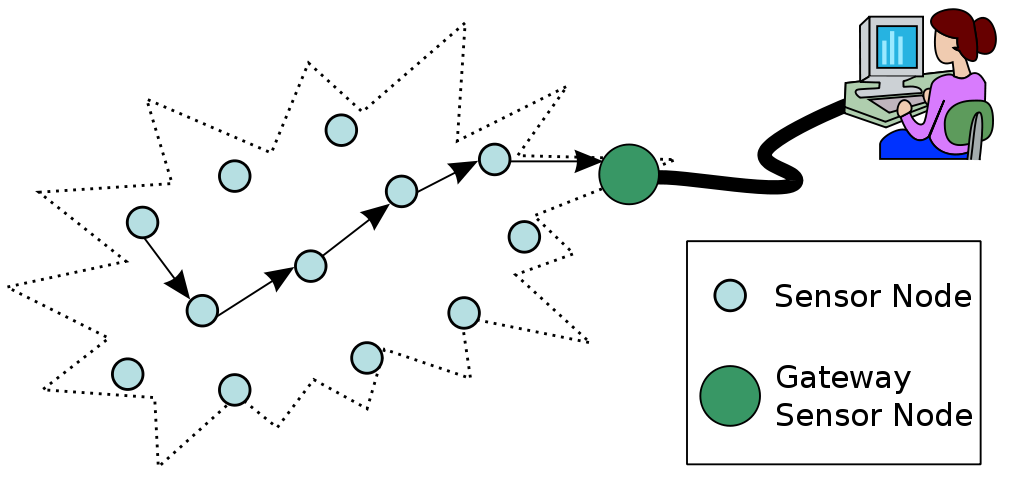
\includegraphics[width=\textwidth]{res/wsn.png}
  \caption{Wireless Sensor Networks (source: \url{commons.wikimedia.org/wiki/File:WSN.svg} )}
  \label{fig:wsn}
\end{figure}

Wireless Sensor Networks are regularly used for environmental conditions monitoring such as wild fire tracking, agriculture management, humidity and temperature monitoring in forests, effect of global warming on glacier structures, air pollution monitoring, and many more. They are also used in the industrial field such as in data centers, mainly to monitor the temperature of racks.  \\

The components of WSNs are "\textit{Wireless Nodes}" or "Motes" (see Fig.\ref{fig:xm1000}). WSNs may be composed of a few hundreds to thousands of nodes, each node being connected to one or several sensors. In addition to sensors, those nodes are also equipped with a microcontroller, a radio transceiver, memory, and a power source (eg. battery). The sensors are responsible for capturing data from the environment, especially when there is a change in an environmental condition such as temperature or humidity. (The continual analog signal produced by the sensors is digitized by an analog-to-digital converter and sent to controllers for further processing). Sensors are usually very small and thus consume a very low amount of battery power. The \textit{microcontroller} is responsible for performing specific tasks and processing the data collected by the sensor, but also controlling other components of the node. The transceiver is used for communication purposes, mainly sending and receiving data using specific. It is often of the form of a radio or infrared. Transceivers have the particularity of both being able to send and receive data. Finally, the power source provides power supply instead of mains supply. The power source is thus in the form of a battery, it is consumed when the node is sending the environment, communicating with other sensor nodes, and doing some data processing. All of the components are designed to be as little power-consuming as possible. Having nodes not connected to mains power is an advantage because of not having to be plugged to a power supply (when the physical world makes it hard to have some, in moutains for example), but with such an advantage come resource constraints as we will explain later.\\

\begin{figure}
  \centering
  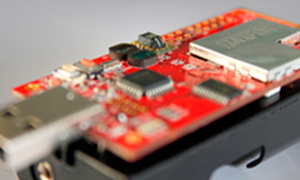
\includegraphics[width=0.5\textwidth]{res/xm1000.png}
  \caption{A AS-XM1000 sensor mote capable of sensing light, humidity and temperature (source: \url{www.advanticsys.com})}
  \label{fig:xm1000}
\end{figure}

The main challenges of WSNs are Data transmission, resource constraint, and security. First, nodes must send their data to the server. As discussed earlier, each node may not have the server in their sending range because of a lack of power, thus they must send their data to an intermediate node relaying the information. Moreover, limited battery, must stay idle, ENERGY HARVESTING etc. Puis security.\\

((((((Each such sensor network node has typically several parts: a radio transceiver with an internal antenna or connection to an external antenna, a microcontroller, an electronic circuit for interfacing with the sensors and an energy source, usually a battery or an embedded form of energy harvesting. A sensor node might vary in size from that of a shoebox down to the size of a grain of dust, although functioning "motes" of genuine microscopic dimensions have yet to be created. The cost of sensor nodes is similarly variable, ranging from a few to hundreds of dollars, depending on the complexity of the individual sensor nodes. Size and cost constraints on sensor nodes result in corresponding constraints on resources such as energy, memory, computational speed and communications bandwidth. The topology of the WSNs can vary from a simple star network to an advanced multi-hop wireless mesh network. The propagation technique between the hops of the network can be routing or flooding.)))))\\

(source : architecting the iot page 6)
(((((
Sensor networks consist of a certain number, which can be very high, of sens- ing nodes communicating in a wireless multi-hop fashion (Figure 2). In general, nodes report their sensing results to a small number of special nodes called sinks (or base stations). A lot of effort has been undertaken by the scientific commu- nity on sensor networks. Indeed, many work have addressed several problems at the different layers of the protocol stack. In these works, the main issues concern energy efficiency (which is a limited resource in WSN), scalability (the number of nodes can rise significantly), reliability (the system might be involved in critical applications), and robustness (nodes might be subject to failure) [17].

\subsection{Radio Frequency IDentification - RFID}

Radio-frequency identification or RFID uses radio signals to record the presence of specific objects. Its purpose is the identification of a person or an item, using a system of tags. Tags are small transponders (combined radio receiver and transmitter). The transponders can transmit identity information when requested to. There also are tag readers to process the identification.\\

Tags are associated to products, animals, or people if their identification is needed for tracking for instance. The tracking is done using radio waves. There are two kinds of RFID tags, the active RFID tags that are battery-powered, and the passive RFID tags that have no batteries and work using signal power from other tags requesting information.\\

The RFID technology has a main advantage that is its limited cost and thus allow its deployment on a huge amount of devices.
\section{Challenges of The IoT}

https://datafloq.com/read/three-major-challenges-internet-of-things/83 : cet article parle de trois gros challenges pour l'iot : shared standards and infrastructures, data control and access, data security.\\

\subsection{Lack of Standard Architecture}

The main challenges of the Internet of Things is to define a standard architecture. This is actually the main reason why it has not been fully deployed yet. Several characteristics are needed for the IoT to be deployed, and they should be included in the standard infrastructure. The characteristics needed are distributivity, interoperability (devices from different companies being able to communicate, with standardized protocols), scalability (huge amount of smart objects communicating), resources scarcity (power and consumption are limited on each device), and security.\\

Most existing applications using the Internet of Things have been developed privately. Companies, developers, researchers have developed some specific solutions using the Internet of Things. However, those solutions are more specific, and hence optimized, for one particular application.\\


Main source : architecting the internet of things : state of the art.\\

\subsection{Three Aspects of The IoT Building Blocks}

As stated earlier, the introduction of the Internet of Things will mostly be an incremental integration to the current Internet. However, the IoT Building Blocks is composed of three particular technologies that are crucial in the deployment of the IoT. First, there is the sensing technologies that are used to gather the interesting data. Then, there is what we call the middleware layer, that processes and manages the raw data gathered from the sensing technologies. Finally, there is the actuating technologies, corresponding to the physical extension of the IoT applications. We will take a look at the impact of these three notions on the future of the IoT.\\

The \textit{Sensing building block} plays an important role in data harvesting and communicating the data collected with sensors. Data is mostly transferred in a wireless fashion, in a Wireless Sensor Networks(WSN) organization or thanks to radio-frequency identification (RFID) because of their ability of sensing the environment. However, those organizations come with a few disadvantages such as security issues, reliability of wireless communication, and especially limited energy consumption that figures as a central obstacle to the deployment of WSNs and IoT networks. The limited availability of energy resources is an important matter to take care of. As a result, lightweight and energy-efficient routing protocols have been proposed but can only mitigate the energy limitation. \\

The \textit{Middleware building block} is a software interface that provides abstraction to hide heterogeneity of the technologies that are used in the Internet of Things and that may indeed differ from each other. Hence, the developers are exempted from having to know how the lower layer of the IoT works, and can primarly focus on the design of applications. \\

The middleware block could be taken care of by what we call \textit{Service-Oriented Computing} approches. A Service-Oriented architecture is a set of communicating services based on standardized interaction models. Associating Cloud Computing with a service-oriented architecture could actually provide an efficient middleware for the IoT. Sensor-clouds are of great help when it comes to handling huge loads of sensed data generated by sensing devices. Thus, approaches based on service lying on a cloud infrastrcuture introduces flexibility and adaptativity to middlewares for the IoT. The idea is to have the end users feel as if the physical sensors were virtually part of their physical resources (in their disk storage, or memory for example). In this case, the users do not need to know the location of the devices nor to know their location, and several end users from different companies developing different applications could exploit the sensors through the cloud. The cloud would thus provide sensor services to be exploited by different IoT applications. All these elements are key to developing IoT applications working on heterogeneous devices. \\

The \textit{actuating building block} finds its importance when it comes to making "dumb" objects "smart". Once information is gathered from sensing in a specific situation, it is sent to the middleware infrastructure. After data processing from the middleware, a decision can be made through the actuator. In our e-health example discussed earlier where an ill person is equipped with an IoT node, in a hypoglycemia situation, the actuator could potentially save this person's life by automatically injecting sugar in the patient, the automation of the injection being faster than the wait needed for external intervention. \\

\subsection{Potential Architecture Design}


\subsection{Existing Architectures}

Even though no global standard infrastructure exists for the Internet of Things, some companies have nevertheless attempted to develop their own architecture, mainly for specific purposes answering to their local needs. We will take a look at some of the existing ones and see what they cannot be a general solution.\\

%%%%%%%%%%%%%%%%%%%%%%%%%%%% IOT OS %%%%%%%%%%%%%%%%%%%%%%%%%%%%%%%%%%%%

\chapter{ContikiOS - Cooja - Softwares a portee de main}

We will now discuss Operating Systems in the Internet of Things. As discussed earlier, objects in IoT Networks have limited capabilities, i.e. processing capacity and storage, and limited battery. It is thus preferred to have an operating system that is not demanding and as light as possible. \\

Though not ideal, a light version of Linux could be used. However, one requirement of working with smart objects is having the ability to react to \textit{Real-Time events}. In a situation where a smart sensor is used in a car to make its airbags open when a car crash occurs, the software in the said sensor must react to the crash almost instantly. In this case, we need a maximum time reaction to an event, otherwise the purpose of the object (and thus the airbag) is not met. A few operating systems have been developed to answer to the requirements of IoT objects, they are light, have a minimal set of functionalities, plus they guarantee time-bounded reaction to events. (source : Mobile and embedded systems, prof Sadre)\\

\todo[inline]{Cite different OS like Tiny OS, RIOT OS}
There exists quite a number of Operating Systems for IoT devices nowadays \cite{website:iot_os}.

\section{The Contiki Operating System}

Among existing operating systems, we have chosen to use one that is called \textit{ContikiOS}. It is an open source operating system and it was developed in 2003. Contiki is quite light in terms of memory, processing speed, and communication bandwidth. It is preemptive.\\

The reason we have chosen Contiki as OS for testing our idea is due to the simulation software, Cooja, which facilitates the debugging and the tests. Another reason, is that we are quite familiar with it having already programmed using Contiki. However, our solution should be easily ported to other OSes. The OS is just used to program the motes.\\

\begin{itemize}
\item protothreads
\item Reduced C
\end{itemize}
wikipedia : "Contiki provides three network mechanisms: the uIP TCP/IP stack,[5] which provides IPv4 networking, the uIPv6 stack,[6] which provides IPv6 networking, and the Rime stack, which is a set of custom lightweight networking protocols designed for low-power wireless networks. The IPv6 stack was contributed by Cisco and was, when released, the smallest IPv6 stack to receive the IPv6 Ready certification.[7] The IPv6 stack also contains the Routing Protocol for Low power and Lossy Networks (RPL) routing protocol for low-power lossy IPv6 networks and the 6LoWPAN header compression and adaptation layer for IEEE 802.15.4 links.

Rime is an alternative network stack, for use when the overhead of the IPv4 or IPv6 stacks is prohibitive. The Rime stack provides a set of communication primitives for low-power wireless systems. The default primitives are single-hop unicast, single-hop broadcast, multi-hop unicast, network flooding, and address-free data collection. The primitives can be used on their own or combined to form more complex protocols and mechanisms.[8]"

\section{Cooja Simulating Software}
An existing tool called \textit{Cooja} has been developed on Contiki. Cooja is a simulation software (partly an emulator too) for Internet of Things networks. It has many features, such as allowing to build networks with different types of components (Sky motes, Z1 motes). Those components are Contiki nodes, i.e. nodes working through ContikiOS. Cooja allows to upload code to virtual motes, the same way Contiki code may be uploaded on physical. Cooja can either emulate nodes (the hardware of each component is entirely emulated), or create "Cooja nodes" where Contiki code is uploaded on, compiled and then executed on a simulation host. (Cooja allows to use non-Contiki nodes as well. Pertinent?). Cooja presents itself as a very useful software for our thesis, as it allows us to simulate large networks, and is quite useful when it comes to testing, since the uploading and compilation time of Contiki codes on the nodes in the Network we are testing and analyzing is faster than on real hardware. It also avoids physical material restriction.

%%%%%%%%%%%%%%%%%% MONITORING TOOLS %%%%%%%%%%%%%%%%%%%%%%%%%%%%%%%%%%%

\chapter{Monitoring tools}

This chapter will be the occasion to present what has been done in matter of monitoring tools for networks. The first section will be about the traditional networks and the second one will be focused on the IoT networks.

\section{Traditional networks}

When speaking of monitoring for traditional networks, two techniques come to mind: \textit{Netflow} and \textit{sFlow}. The two approaches have the common goal to give network administrators informations about the traffic that passes through their networks. However, they differentiate in the way they do so. In our solution, we were mainly inspired by Netflow as it is lighter than sFlow in term of memory used.

\subsection{Netflow - A Traffic Collector}

\textit{Netflow} is a feature that was created by Cisco Systems and introduced on Cisco Routers. Netflow allows the collection of the IP traffic in networks, and thus monitoring network traffic. Information such as Source and Destination addresses (defined as "Flows) and Traffic volume can be retrieved and further analyzed.\\

There are three components when having Netflow set up : the Flow Exporter, the Flow Collector(s), and the analysis application. The Flow Exporter collects packets and forms what we call flows (having various definitions according to the version of Netflow used). Flows represent a stream of packets sharing common attributes (such as source and destination addresses). The exporter records the flows into Netlow records and sends passes them onto the Flow Collector. After reception, the Flow Collector will store the flow records received from the Exporter. The data stored can then be analyzed by applications, hence having statistics of traffic exchanges in a particular network. This process is illustrated in Fig.\ref{fig:netflow}.\\

\begin{figure}
  \centering
  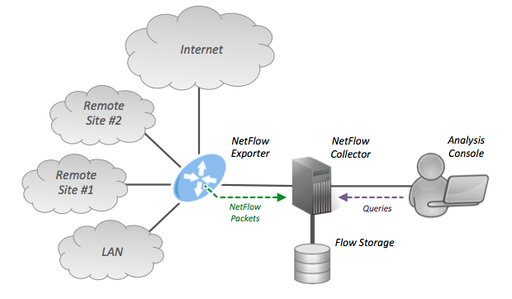
\includegraphics[width=\textwidth]{res/netflow.png}
  \caption{Netflow}
  \label{fig:netflow}
\end{figure}

The version of Netflow that we are quite interested in, is the Netflow version 10 or \textit{IPFIX} \cite{claise2013rfc}. This version is an IETF (Internet Engineering Task Force) protocol whereas the previous versions are proprietaty protocols of Cisco. IPFIX is template based meaning that contrary to previous versions of Netflow (excluded version 9 which is also template based), the netflow records can vary to suit the need of the administrators or organizations. The template permit to define what we want to retrieve and by the same occasion define what we consider to be a flow. An organization could consider a flow to be 3-uple: source ipv6 address, destination ipv6 address, number of octets exchanged. While another one could consider a flow to be the 4-uple: source ipv6 address, destination ipv6 address, number of octets exchanged, number of packets exchanged. \\

\todo[inline]{Ajouter figure de IPFIX}.\\
The IANA (Internet Assigned Numbers Authority) defined already some record fields like the Ipv6 source/destination address, the source transport port, and so on \cite{website:ipfix_entities}. However, the power of IPFIX lies in the possibility to define ourself record fields (called entreprise fields). And that is the main reason we were so interested in it. It is thus possible to define for example a record field for battery remaining of the sender for example. Furthermore, even if they suggest size for record fields, they offer the possibility to redefine the size to a smaller one. The suggested field is only considered as an upper-bound, meaning we cannot propose a bigger size.\\

Having defined what Netflow is, the main goal here is to be able to use Netflow on an IoT device. In the Introduction section, we explained that our main goal was to analyze the traffic of an IoT Network and retrieve pertinent information such as the volume exchanged in the network, and its topology. Netflow is basically what we want to achieve in terms of data collecting. However, it has not been implemented by Cisco for IoT devices. Our task is to implement Netflow for an IoT device, using predefined data formats that will allow us to collect the information we are interested in (battery level, source and destination addresses, packet volume, etc.). In the Part \ref{part:solution}, we will describe in more details how we used Netflow in IoT Networks as a solution to our monitoring task.

\subsection{sFlow}

\textit{sFlow} (for sampled flow) was initially proposed by the company HP. It is maintained by the sFlow.org consortium \cite{website:sflow}. The approach taken by SFlow is different than the one taken by Netflow. The two solutions shares the notion of exporter, collector and analysis application. But the difference is in the records that are sent by the exporter. \\

Whereas Netflow sends only informations on the flows observerd, sFlow sends original packets that pass through the network. sFlow is characterized by the \textit{polling interval} and the \textit{sampling rate}. The polling interval defines the periods at which the collector must report the number of occurences of packets that pass through. The sampling rate defines how much packets need to be sampled on a set number of packets. \\

The fact that exporters need to store packets makes this solution too heavy for majority of IoT devices. Another issue with sFlow is that we can miss peculiar packets by having a sampling rate different than 1:1 and so lose important informations.

\section{IoT networks}

A plethora of tools exist to monitor Internet of Things networks. Yet, a preponderant part of those tools are data visualization centric. In this section, some tools will be presented. For a more exhaustive survey, see \cite{parbat2010data}.

\subsection{Octopus}

\textit{Octopus} \cite{jurdak2011octopus} is a software that permits to monitor and visualize WSN networks. It offers also the possibility to control those networks by giving command. The software was written in Java. \\

The GUI interface, Fig.\ref{fig:octopus_gui}, display a logical topology of the sensor nodes as well as charts reporting the retrieved values from the nodes. It also enable an user to modify the sampling rate at which nodes report the environmental values. \\

To effectively do so, Octopus needs the motes to send message in a specific format so as to be able to parse them. Also the motes need to be configured to be able to interpret messages coming from the software.\\

The architecture of Octopus, Fig.\ref{fig:octopus_archi}, is straightforward. The sensors nodes send periodically messages to a gateway which will be in charge to transmit those messages to distant Octopus client. The Scout can be seen as collector that will listen for incoming messages. When it received a message, it will update the Mote DB who is in charge to maintain the status of the motes and also log the message. It will also trigger an update of the GUI interface, Panels.

\begin{figure}
    \centering
    \begin{subfigure}[b]{0.5\textwidth}
      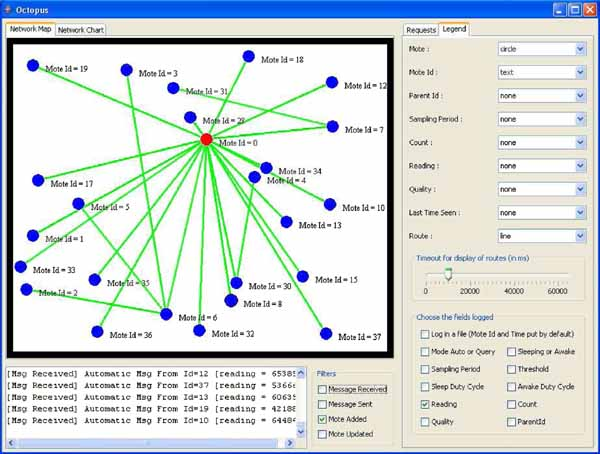
\includegraphics[width=\textwidth]{res/octopus.png}
      \caption{Octopus GUI}
      \label{fig:octopus_gui}
    \end{subfigure}
    ~
    \begin{subfigure}[b]{0.5\textwidth}
        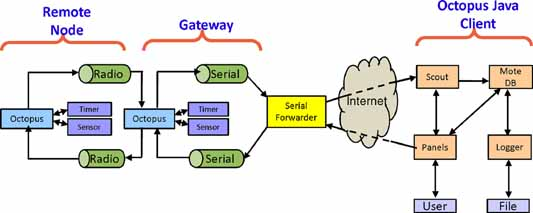
\includegraphics[width=\textwidth]{res/octopus_archi.png}
        \caption{Octopus architecture}
        \label{fig:octopus_archi}
    \end{subfigure}
    \caption{Octopus (Source: \url{www.researchgate.net/publication/220098661_Octopus_Monitoring_visualization_and_control_of_sensor_networks})}
    \label{fig:octopus}
\end{figure}

\subsection{Spyglass}
\todo[inline]{Explain}
\textit{Spyglass} \cite{buschmann2005spyglass}.

\subsection{Foren6}

The approach taken by Cetic with their tool \textit{Foren6} \cite{website:foren6} is quite different than the other tools presented. Foren6 use a sniffer to retrieve information of the network. Passive sniffers are scattered over the network and retransmit the traffic they observe. \\

The Fig.\ref{fig:foren6} shows the GUI interface of Foren6. Foren6 dispose of the following features:
\begin{itemize}
  \item Display logical topology of the motes.
  \item Analyze of previous records packet traces.
  \item Possibility to analyze simulated network like with Cooja. \\
\end{itemize}

\begin{figure}
  \centering
  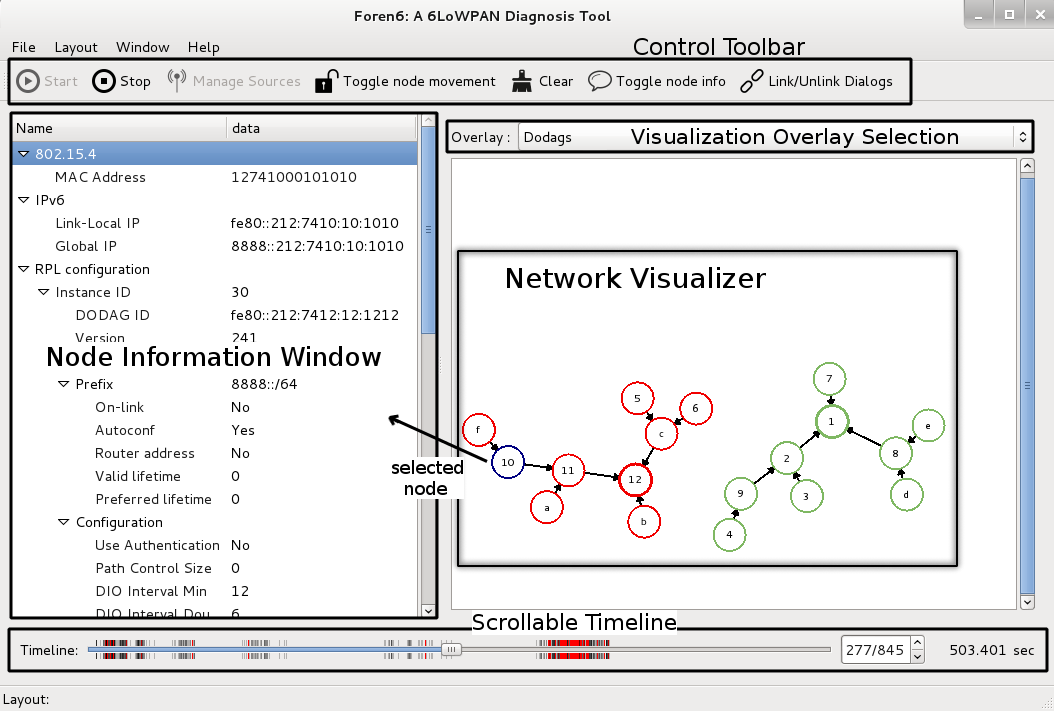
\includegraphics[width=\textwidth]{res/foren6.png}
  \caption{Foren6 GUI (source: \url{cetic.github.io/foren6/})}
  \label{fig:foren6}
\end{figure}

To be as efficient as possible, the solution offered by Cetic needs nodes to be solely focused on sniffing and also present enough processing power and battery to be able to sniff and transmit the packets captured. If the network is deployed on a large surface, there will be a need to have enough sniffers, well placed, so as to not miss traffic. Also should those motes, sniffers send the packets captured using IoT network monitored, it would increase the burden on the latter network.

\part{Solution} \label{part:solution}

\chapter{IoT Monitoring Tool}

This chapter will be the occasion to detail the architecture of our solution. We will explain the technologies employed to achieve our goal, a monitoring software for Internet of Things networks. It is also in this chapter that we will justify the choices we made during the development of it.

\section{Architecture}

The architecture of our solution is composed of two parts as can be seen on Fig.\ref{fig:design}. The first part is about how the data is collected and sent. The second part consists of how the data is received and treated after reception. In the remaining of the section, strong assumptions are made that the reader is familiar with Netflow, particularly IPFIX, also referred as Netflow v10, and also its implementation for WSN which is called TinyIPFIX. If not, explanations about those particular technologies can be found in Chap \ref{chap:monitoring_tools}. \\

\begin{figure}
	\centering
	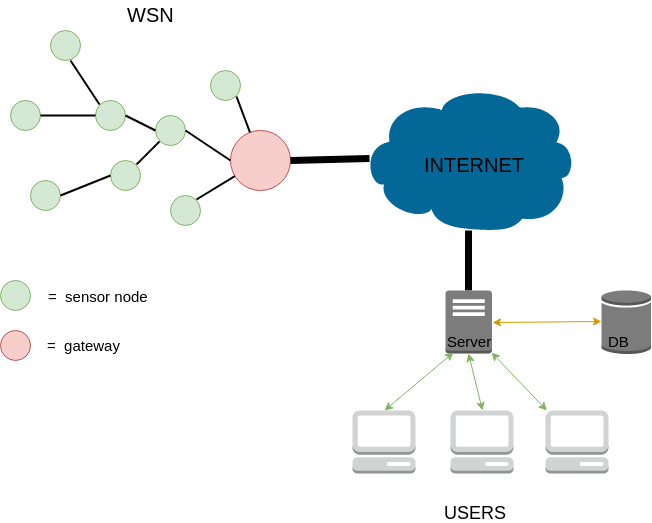
\includegraphics[width=0.8\textwidth]{res/design.png}
	\caption{Global architecture of the solution}
	\label{fig:design}
\end{figure}

The data exportation is done in a Netflow fashion. The nodes occupy the role of exporters. Each node maintains a flow table where they register the flows that occurred during an interval of time. In our case, a flow is characterized by the 4-uple: source node id, destination node id, number packets and number octets. After a certain amount of time, each node will construct a TinyIPFIX message based on the content of its flow table. Those messages are sent to the gateway node. The gateway node will then reformat the TinyIPFIX messages received into compliant IPFIX messages to a specific address, which will be in our case the address of a server. The messages are sent using UDP. It is not reliable but using TCP to transmit data would incur the cost of initiating the connection and closing it. Also in a reliable network with a high packet loss percentage, resending information would increase the load on the nodes.\\

The server that receives the IPFIX messages from the IoT network plays two roles. One role is straightforward, it plays the role of collector. Each message is collected by the server and logged in a database for further processing and analyzing. The other role is of a web server. Multiple users can know the network status by having access to web pages served by the server.

\section{Technologies}

The monitoring tool developed for this thesis is a \textit{web-based} solution. We've chosen to write the monitoring tool with \textbf{Node.js} \cite{website:nodejs} which is a server-side solution for Javascript. In that sense, it offers modules or API to effectively develop HTTP/HTTPS server, meaning web server. To speed up our development, we used the \textit{Express framework} \cite{website:express} on top of Node.js. Express simplify the routing of requests to views. A view can be seen as an web page. \\

The reasons we've chosen to write our monitoring tool as a web-server is the portability of such a solution. All OSs dispose of a web browser. For the user, it simplifies the utilization of the tool by simply accessing the web site via its preferred browser. The user does not have the trouble to download and install our software as with common desktop applications. Also, the user can freely access the tool from different locations and computers. He is not limited to devices where the software is installed on. \\

Another factor in favor of a web solution is the ease with which multiple users can access the software in the same time. Most of the monitoring tools presented are desktop applications. They take the role of collectors and store the logs in a local database. This implies that the nodes transfer their data directly to the device having the monitoring tool on. However, a considerable drawback of such design is when multiple administrators exist for a same IoT network. Multiple users are bound to one device to monitor the network. One approach would be to retransmit the data sent by the nodes to each devices containing the monitoring tool in question, but it does not scale well. The web solution is not limited by that. By having a centralized server playing the role of collector but also of web server, different users can efficiently monitor the network on their own device by simply requesting the web server. \\

One of the reasons for developing the software with Node.js and not other particular frameworks like Django or Ruby on Rails is due to the features that it offers via notably the Javascript language. First, it is event-driven and asynchronous by nature which is what we desire for our product. One such event to react to is when the collector receives an IPFIX message. Other events are when the status of a node changes as you will see later on. Programming by events proved powerful in our case. Secondly, the huge support on the Javascript language and its popularity which makes it a good choice for the adoption of the tool. Additionally, the huge documentations and modules helped us develop the tool faster and better. Thirdly but nonetheless, Javascript is tightly coupled to JSON (Javascript Object Notation) \cite{website:json} which is a data-interchange format. Objects in Javascript can be easily formated to JSON formated and exchanged via Internet. This allow to make dynamic website. Finally, we limit the language used during the process of production of the software mainly to Javascript for backend and HTML, CSS and Javascript for frontend where other frameworks would impose to master one or two more languages.\\

HTML, CSS and Javascript which are the core means to present web pages proved to be useful but also easy to produce ways of visualizing the data. Javascript presents a lot of library to display graphs, charts and other type of figures. One such popular library is D3.js \cite{website:d3}. It also enables a website to be dynamic. Popular libraries like Bootstrap helped in making web page quicker and saved us the trouble to modify CSS files.\\

For the database, \textbf{PostgreSQL} \cite{website:postgresql} was used. It is an open-source relational database system. With more than 15 years of development, it does not have to prove anything anymore in term of reliability. It is SQL compliant. It recently added the support of JSON as field which enabled us to save IPFIX messages as JSON objects and not simply binary data.

\section{The monitoring tool}

This section will detail the different modules that compose our application plus the features that are offered by our application.

\subsection{Modules}

The application is comprised of four different modules :
\begin{itemize}
	\item Collector
	\item Log
	\item Nodes Status
	\item Web \\
\end{itemize}

The \textit{Collector} consists of a UDP server that listens to incoming IPFIX messages. Upon reception of a message, the Collector parses the binary data into an IPFIX object representing the original message. The object created is what will be used for the application to work with. It offers methods to read records contained in the original IPFIX object. The Collector emits an event each time it creates an object from a received message. Modules can then listen and react to this particular event and treat the newly created object. \\

The \textit{Log} module offers logging capabilities of IPFIX message. It also gives the possibility to query it. The storing is done in a PostgreSQL database. However, users can freely switch to its SQL prefered database as long as it also offers the possibilty to create a JSON field. To log an IPFIX message, it listens to the Collector's event mentioned before. It then stores in the database the JSON representation of the object. The module proposes methods to query the database such as having the different flows between two nodes as example. As to enhance the reactivity of our application, other tables are created apart from the ones that contained the IPFIX objects. One such table is the different flows.\\

To keep track of the status of the nodes, we deemed necessary to create a \textit{Nodes Status} module. This particular module also listens to the Collector's event for incoming IPFIX object. It will then update the status of the nodes according to the content of the object. The status of a node comprises its parent, its battery, its number of bytes sent, number of packets sent and the last packet sent, to name a few. The Nodes Status module offers the current state of the different nodes contained in the IoT network. To retrieve past values, it is necessary to pass via the Log module. \\

The final module is the \textit{Web} one. This module is essentially an HTTP server. Users interact with our tool mainly via this module. It permits users to visualize the status of their network via their browser by launching HTTP requests to which the server will reply by delivering the requested content. This module is an intermediate between the users and the Nodes Status module but also between the users and Log module. The reason for that is, to deliver content to the users, this module needs to gather data which is contained by the two aforementioned modules. This module can be seen as the frontend of our application whereas the others can be viewed as composing the backend of our solution.\\

The reasons behind using multiple modules is to achieve one of the requirement we imposed on ourselves, the \textit{modularity} of our program. We stated that a user should easily extend our software to add new features. By separating our applications into four different modules, we achieved this requirement. Each module offers different functionalities and abstractions. The Collector is responsible of collecting the IPFIX messages, the Log module to log those messages and provide means to query the logs, the Nodes Status keeps track of the status of the IoT network and finally the Web module permits users to interact and visualize the data. Users wanting to add new web pages will mostly only have to look into the Web module by adding another route to which the server will respond by replying by an HTML page. \\

The Fig.\ref{fig:modules} depicts the different modules presented and their interactions. As shown in the figure, the modules occupy different layers. The first layer is occupied by the Collector. The second one is occupied by the Nodes Status and Log modules. And finally the third one is composed solely of the Web module.

\begin{figure}
	\centering
	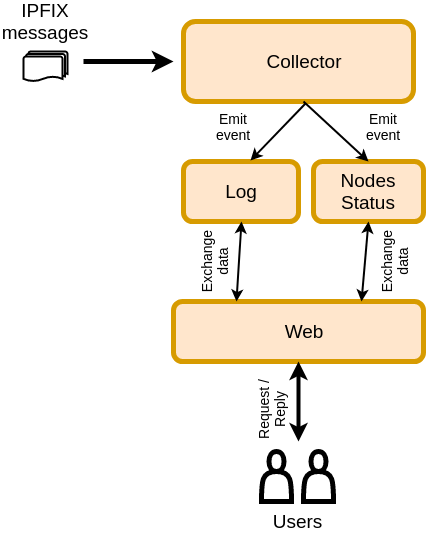
\includegraphics[width=0.5\textwidth]{res/modules.png}
	\caption{Modules interactions}
	\label{fig:modules}
\end{figure}

\subsection{Features}

The features offered by our monitoring applications are what we considered to be the basic ones. More description will be done on the next chapter.

\begin{description}
	\item[Topology Map] Display the logical topology of the WSN. The topology represents the RPL routing, meaning the topology is actually acyclic and represents a tree. A link represents a relation of parent-child between two nodes. The root is the gateway node, and is colored differently to distinguish it from leaf nodes, which do not have children. Each node composing the topology is associated with its unique respective ID. Moreover, those nodes are uniquely clickable, one at a time, to get further information about their node values.
	\item[Node values] Offers the possibility to see more in depth the values sent by a particular node. With these features, an administrator has the possibility to see how the different values have evolved in time. It also gives meaningful statistics as the average number of bytes sent by interval of time, how often it is addressed and so on.
	\item[Network statistics] Gives statistics which are general to the whole network. This comprises the amount of traffic generated by the network. But also gives meaningful insight about the node having the less battery or the node sending the most data. This gives a broad view to the administrator.
\end{description}

\chapter{The Monitoring Tool - A web interface}

In this chapter, we will showcase and explain the features of our Monitoring software. As stated earlier, we have built a web interface for the monitoring of IoT networks. There are two main tabs, one that showcases \textit{traffic volume} evolving through time, and the other one that shows the \textit{topology} of the IoT network under visualization.

\section{Traffic Volume}

The Traffic Volume page shows how the traffic evolved during time for a particular network. As can be seen on Fig.\ref{fig:tool_traffic}, this page is divided into six different panels. \\

The first panel contains a graph that shows evolution of the traffic in term of bytes over time. More precisely, we consider interval of 5 minutes. This graph contains two lines. The blue one is for normal traffic and the other one, in orange, is for IPFIX traffic. Normal traffic is all traffic that is not Ipfix nor TinyIPFIX. With that, administrators can see if the bytes generated by the monitoring with TinyIPFIX is of great importance or not. \\

The second panel, top right, is a brief summary of the network. It shows how much bytes and packets were sent. But it also shows the average packet size. Those number are computed for three type of traffics: IPFIX/TinyIPFIX traffic, normal traffic and also normal plus IPFIX/TinyIPFIX traffic.\\

The third panel, bottom left, shows statistics about the IoT network. Those statistics are the minimum and maximum bytes generated for a particular interval. It also give information about the average number of bytes sent by interval. Those statistics are only computed on normal traffic. Deduction is thus done of the IPFIX/TInyIPFIX traffic.\\

The fourth panel is a pie showing the repartition of the total traffic. It shows the repartition of the traffic between IPFIX messages, broadcast messages and unicast messages. Broadcast messages are often used in networking for networks to organize  themselves like finding neighbors, assigning addresses or routing purposes. By showing the proportion of broadcast messages, administrators can have an idea about the amount of data sent for the IoT network to structure itself.\\

Finally the fifth and sixth panels shows the top five source and top five destination respectively. The top source are the the nodes that sent the most data while the top destination are the nodes that receives the most bytes. It permits to quickly see if a node presents, for example, a too much number of bytes sent compare to other nodes or if a node is contacted too often.

\begin{figure}
	\centering
	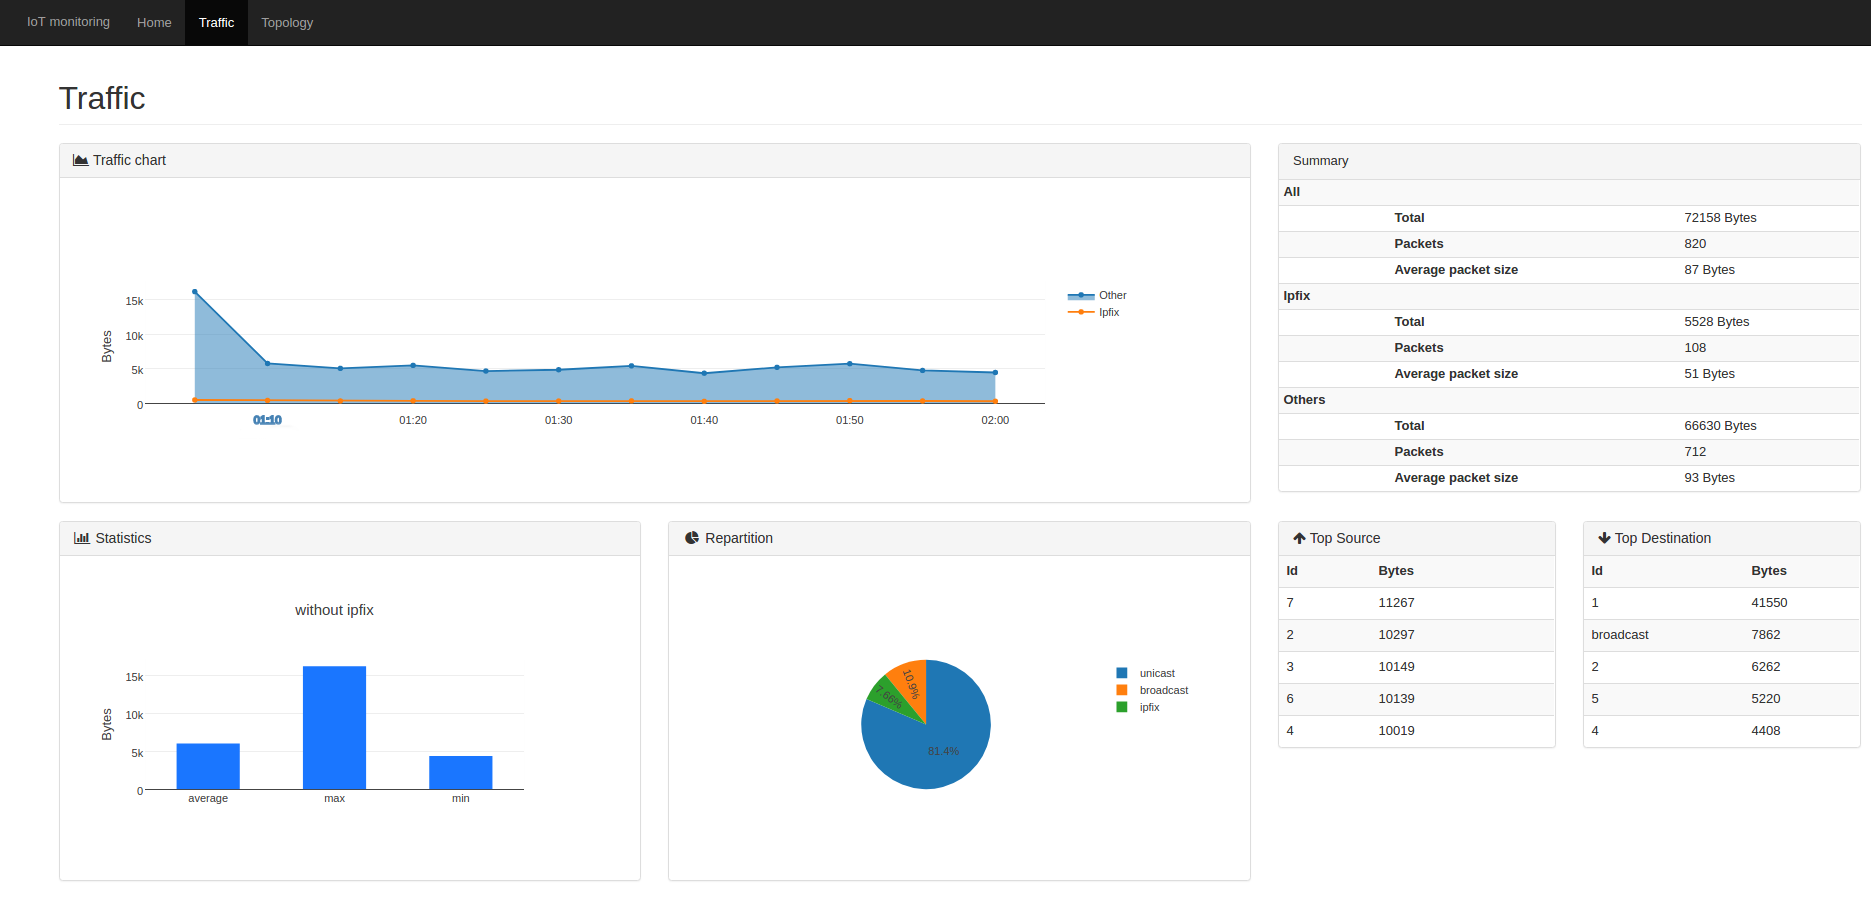
\includegraphics[width=\textwidth]{res/traffic.png}
	\caption{Traffic Volume}
	\label{fig:tool_traffic}
\end{figure}

\section{Current Topology}

\begin{figure}[!h]
	\centering
	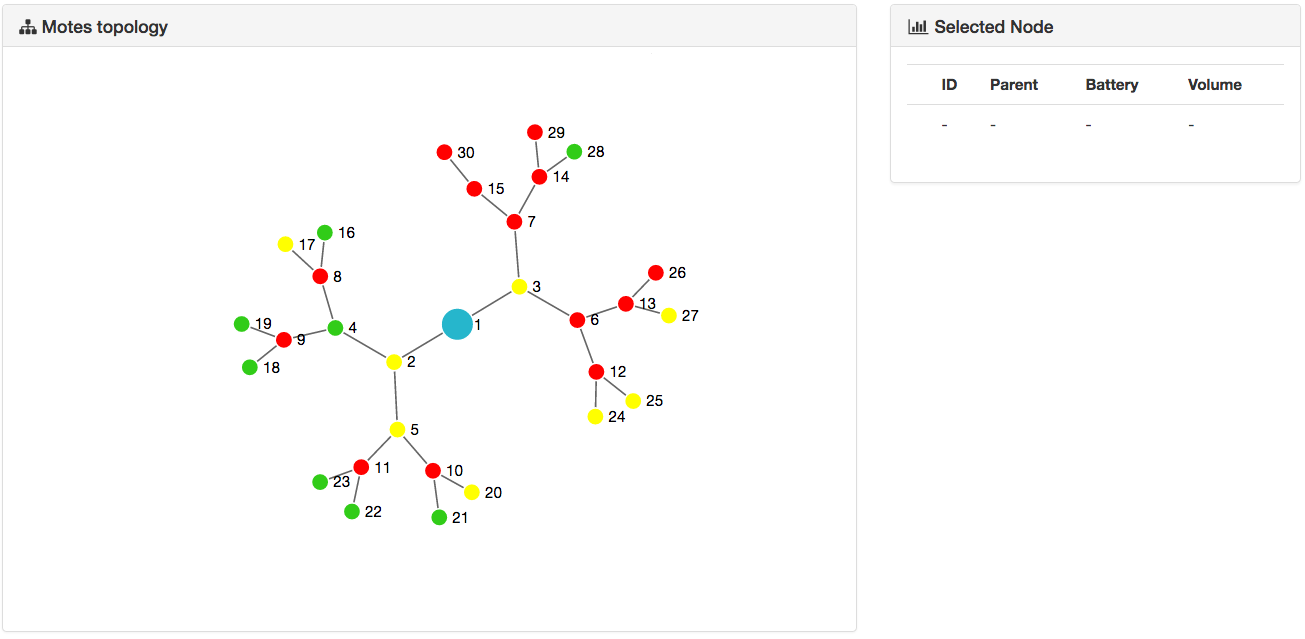
\includegraphics[width=1.1\textwidth]{res/topologyinterface.png}
	\caption{Topology Tab}
	\label{fig:topo}
\end{figure}

In this tab, lies the topology of the network that is under visualization. Once all the traffic data has been received and processed by the server, it becomes possible to see the topology of our IoT network. As you can see in figure \ref{fig:topo}, the \textit{Motes topology} zone is where the graph is shown. \\

Evidently, each node is represented as a circle, the \textit{gateway mote} being slightly larger and in sky blue. and each grey link represents a connection "parent to child" in the IoT network. All nodes in the topology are clickable, one at a time. It is not possible to click on a node if another node is already selected. Once a node is clicked on, its circle becomes larger and is filled in blue, as you can see in figure \ref{fig:snodeblue}. The \textit{Selected Node} panel (figure \ref{fig:snode} (either on the right or under the topology zone according to the browser's window size) allows to display specific information about the node we are interested in, namely its ID, its parent, its current battery level, and the total volume of data it has sent. Note that the Node \textbf{1} is the gateway mote of the netowrk, it thus has no parent and its \textit{Parent} field is filled with "none", for other nodes it would contain another ID.\\

As for the three different colors for regular nodes, we have decided to use them as indicators for battery levels, a node in green has more than 50\% of battery, a node in yellow lies between 50 and 20, and a node in red is below 20\%. The colors could be used for other indicators in the network and with more tresholds, such as the total volume sent, or last time a node has sent information.\\

\begin{figure}[!h]
	\centering
	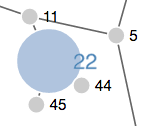
\includegraphics[width=0.6\textwidth]{res/snodeblue.png}
	\caption{Topology Tab}
	\label{fig:snodeblue}
\end{figure}


\begin{figure}[!h]
	\centering
	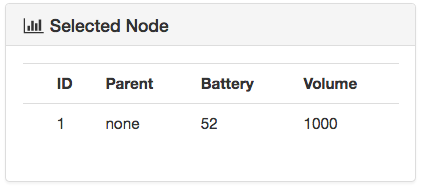
\includegraphics[width=0.6\textwidth]{res/snode.png}
	\caption{The panel showing specific data for a node}
	\label{fig:snode}
\end{figure}



\subsection{The Dragging feature}

\begin{figure}[!h]
	\centering
	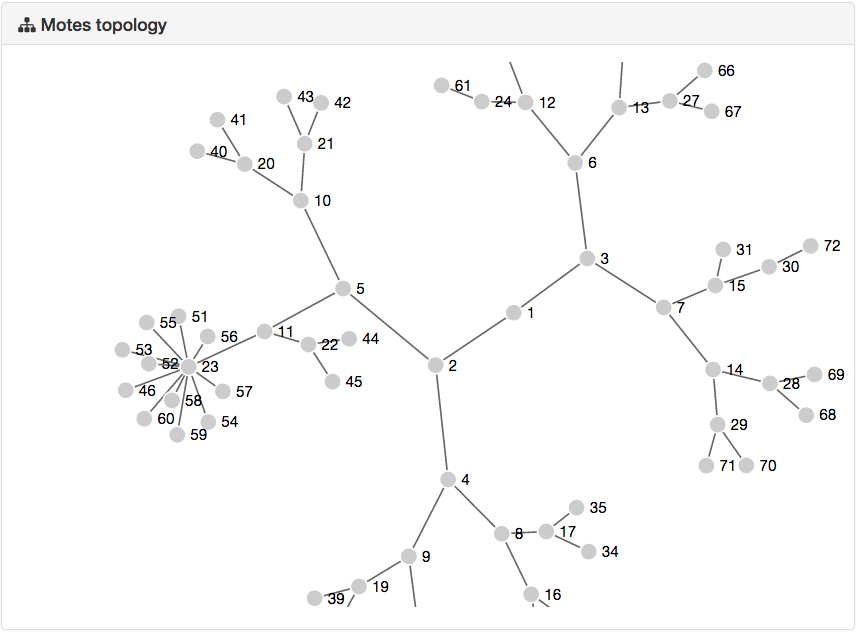
\includegraphics[width=0.6\textwidth]{res/populated.png}
	\caption{The panel showing specific data for a node}
	\label{fig:populated}
\end{figure}


We have decided to implement a dragging feature. That is, by clicking on a node and holding the click, it is possible to move the topology with the direction of the user's mouse. While this feature seems insignificant, it finds its use when the topology gets populated. When there are more than 30 nodes (figure \ref{fig:populated}), the topology may expand further than the borders of the zone dedicated to the topology, as seen in figure \ref{fig:outnode}.



\begin{figure}
    \centering
    \begin{subfigure}[h]{0.3\textwidth}
        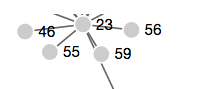
\includegraphics[width=\textwidth]{res/outnode.png}
        \caption{Out of borders nodes}
        \label{fig:outnode}
    \end{subfigure}
    ~
    \begin{subfigure}[h]{0.3\textwidth}
        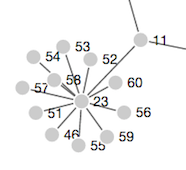
\includegraphics[width=\textwidth]{res/visible.png}
        \caption{Visible with dragging}
        \label{fig:visible}
    \end{subfigure}
    \caption{Dragging result}\label{fig:dragging}
\end{figure}
As you can see in figure \ref{fig:visible}, it is thus possible to fully see any group of nodes, since the topology zone is not unlimited in size. \\



\part{Analysis}  \label{part:analysis}

\chapter{Methodology}

In this chapter, we will present the methodology used to analyze our solution. Our tests were focused on the data retrieval as we considered it to be the part that needed to be evaluated the most. This is mainly due to the fact that our solution will be considered viable only if it do not stress intensively the network. Because we are talking about Internet of Things, and particularly Wireless Sensors Network, preserving the battery life of nodes is a must. This can be done by maximizing the CPU sleep time, or reducing the transmission or reception time. For those particular reasons, five criteria designed our tests:

\begin{itemize}
  \item CPU duty time
  \item CPU low power mode time
  \item Radio transmission time (Tx)
  \item Radio reception time(Rx)
  \item Amount of packets induced by our solution \\
\end{itemize}

The four first arguments can give an estimate of the energy consumption. With that we can build a model to tell whether if our solution depletes the battery too much. Dunkel et al. \cite{dunkels2007software} demonstrate that energy consumption can be given by the following formula

\begin{equation}
  E = (I_m t_m + I_l t_l + I_t t_t + I_r t_r) * V
\end{equation}

where $I_m$ and $t_m$ represents the current draw of the microprocessor when running and the time in which it has been running respectively. $I_l$ and $t_l$  are the current draw and the time of the microprocessor in low power mode. $I_t$ and $t_t$ are the current draw and the time of the communication device in transmit mode while $I_r$ and $t_r$ are the current draw and the time of the communication device in receive mode. Finally, $V$ is the supply voltage. The $I_m$, $I_l$, $I_t$, $I_r$ and $V$ values are device dependent. Different models can present different values. The Tab.\ref{table:device_consumption} shows such values for different models.\\

\begin{table}
  \centering

  \begin{tabular}{|c|c|c|c|c|c|}
    \hline
    Model & $I_m$ (mA) & $I_l$ (mA) & $I_t$ (mA) & $I_r$ (mA) & $V$ (V)\\
    \hline
    Zolertia Z1 & 5 & 0.0005 & 17.4 & 18.8 & 3 \\
    \hline
    Tmote Sky & 1.8 & 0.0545 & 19.5 & 21.8 & 3 \\
    \hline
  \end{tabular}
  \caption{Devices electrical characteristics}
  \label{table:device_consumption}
\end{table}

To implement our benchmarks, we used the couple Contiki-OS and Cooja. The former was used to configure the nodes while the latter was used to simulate those nodes. For more details on those two, see Chap.\ref{chap:contiki}.\\

This chapter will be organized in two sections. First, we will explain the different configurations (number and role of nodes) used for our benchmarks. Secondly, we will explain in more detail the mechanisms used for nodes to send their data. The code used to implement those parts can be found on our public repository \textit{\href{https://github.com/edd19/netflow_contiki}{netflow\_contiki}} on github.

\section{Configurations}
\todo[inline]{explain packet rate}
Four different configurations were used for the purpose of our tests. They all differ by the facts that nodes send IPFIX messages or TinyIPFIX messages  or simply none. However they all share the common components of WSN: sensor nodes and gateway node.

\begin{description}
  \item[Simple] In this configuration, the nodes do not send information about the flows they observed or any meta information about their network. They only occupy the role of sensor nodes, meaning sensing the environment and transmitting the values observed.
  \item[Ipfix] This configuration is an upgrade of the previous one where the nodes now send informations about the flows they observerd. Those informations are formatted using the full IPFIX format. The gateway node do not need to do any conversion and the data is hence transmitted directly to the collector.
  \item[TinyIpfix] This configuration is also an upgrade of the \textit{Simple} configuration. The nodes send flows informations but using the TinyIPFIX format. This imply that the gateway node do conversion of TinyIPFIX to IPFIX before transmitting the data to the collector.
  \item[Aggregation] This last configuration adds aggregators to the \textit{TinyIpfix} configuration. Aggreagators collect TinyIPFIX messages and merge them in one message. They then send those merged messages to the gateway who will convert them to compliant IPFIX messages. In return the gateway node will send the converted messages directly to the collector. \\
\end{description}

The Tab.\ref{table:configurations} resumes the different configurations used during our benchmarks. \\

\begin{table}
  \centering
  \begin{tabular}{|c|c|c|}
    \hline
    Configuration & Monitoring deployed & Aggregator \\
    \hline
    Simple & None & No \\
    \hline
    Ipfix & IPFIX & No \\
    \hline
    TinyIpfix & TinyIPFIX & No \\
    \hline
    Aggregation & TinyIPFIX & Yes \\
    \hline
  \end{tabular}
  \caption{Configurations used}
  \label{table:configurations}
\end{table}

We tested each configuration with an increasing number of nodes of 5, 10, 15 and 20. Each configuration was tested for 25 minutes. The number of nodes was limited by the computer used during benchmarking as it proved unable to simulate more than 20 nodes with Cooja. We also tested the influence of the sending time of the IPFIX messages with a 1 and 5 minutes interval between each message.\\

Also for each simulation we keep track of the following informations:
\begin{itemize}
  \item The 4-uple (Rx, Tx, Cpu, Lpm) where Rx is the radio reception time, Tx the radio transmission time, Cpu the time the Cpu is working and Lpm the time the Cpu is sleeping. This 4-uple was recorded for each minute. This gave an idea on how the energy consumption evolves minute by minute.
  \item A log of all the packets sent during the simulation thanks to a Cooja plug-in. This permits to have an idea on the amount of traffic generated by our solution.\\
\end{itemize}

Our tests were done solely on simulation using the Cooja simulation software. The nodes used during the simulations were the Zolertia Z1. Also we considered a setup for all configurations were the radio loss was null. Also all motes were fixed meaning they did not move during the simulation.

\section{Sending of data}

This section will answer the questions relative on how the motes send IPFIX/TinyIPFIX messages, what triggers the sending of those meta informations and what particular informations are sent. Distinction must be done on the three types of motes: exporter, aggregator and gateway.\\

\begin{description}
  \item[Exporter] It is straighforward. It first send the templates then set a timer. When the timer expired or when the flows table reached its maximum capacity, the exporter exports the records. All packets, templates or data, are sent whether directly to the gateway or to an aggregator node depending on the configuration. The Alg.\ref{algo:exporter} is the algorithm corresponding to an exporter.

  \begin{algorithm}
    \textbf{Function} Exporter:\\
    send templates\;
    set timer\;
    \While{true}{
      yield process until event\;
      \If{timer timeout or flows table is full}{
        send data/records\;
        empty flows table\;
        reset timer\;
      }
    }
   \caption{Exporter algorithm}
   \label{algo:exporter}
  \end{algorithm}

  \item[Aggregator] It is an extension of the Exporter. It both merge and send TinyIPFIX messages. At first it send the templates used then also set a timer. When the aggregator received an TinyIPFIX message, it merged that one with previous ones if any. When a timeout of the timer occured or when the flows table of the aggregator reached its limit, it will merge its records with the ones received then will send the new formed message to the gateway. This behavior is shown by the Alg.\ref{algo:aggregator}.

  \begin{algorithm}
    \textbf{Function} Aggregator:\\
    send templates\;
    set timer\;
    \While{true}{
      yield process until event\;
      \If{received TinyIPFIX message}{
        merge message with previous ones\;
      }
      \If{timer timeout or flows table is full}{
        merge aggregator data/records with received ones\;
        send merged messages\;
        empty flows table\;
        reset timer\;
      }
    }
   \caption{Aggregator algorithm}
   \label{algo:aggregator}
  \end{algorithm}

  \item[Gateway] It convert TinyIPFIX messages received into IPFIX message. The converted messages are sent directly to the collector. This is shown by Alg.\ref{algo:gateway}.

  \begin{algorithm}
    \textbf{Function} Gateway:\\
    \While{true}{
      yield process until event\;
      \If{received TinyIPFIX message}{
        convert into IPFIX message;
        send converted message;
      }
    }
   \caption{Gateway algorithm}
   \label{algo:gateway}
  \end{algorithm}

\end{description}

Two templates were used during our tests. The first template (Tab.\ref{table:traffic_template}) was used to send traffic information about the network while the second one (Tab.\ref{table:meta_info_template}) to obtain meta-information about nodes. The first template considers records of size of 8 bytes. Each record contains the source node id, the destination node id which is the receiving end of a flow and also the number of octets for that particular flows plus the number of packets. This template is the most often used. The second template with records of size of 5 bytes is comprised of the source node id but also the parent node id (in RPL routing) and also the remaining battery of the node. This template is not sent often. It must be sent on update of the parent or at interval of one hour. The fields source node id, destination node id, parent node id and battery were defined for the purpose of this thesis. They are not standard ones.

\begin{table}
  \centering
  \begin{tabular}{|c|c|}
    \hline
    Source Node Id & 2 bytes \\
    \hline
    Destination Node Id & 2 bytes \\
    \hline
    Octets delta count & 2 bytes \\
    \hline
    Packets delta count & 2 bytes \\
    \hline
  \end{tabular}
  \caption{Traffic template}
  \label{table:traffic_template}
\end{table}

\begin{table}
  \centering
  \begin{tabular}{|c|c|}
    \hline
    Source Node Id & 2 bytes \\
    \hline
    Parent node id & 2 bytes \\
    \hline
    Battery & 1 byte \\
    \hline
  \end{tabular}
  \caption{Meta-information template}
  \label{table:meta_info_template}
\end{table}

\chapter{Results}

After having presented our methodology used when testing our solution, this chapter will present and discuss the results obtained from it.

\section{Energy consumption}

The Fig.\ref{fig:average_energy} shows the average energy consumption in term of mJ by minute for the nodes. The bar charts shows the evolution of the energy consumption with increasing number of nodes (5, 10, 15 and 20) for the three configurations \textit{simple}, \textit{tipfix} and \textit{aggrega}. As a reminder, the \textit{simple} configuration has no monitoring done with TinyIPFIX while the two has monitoring activated by the mean of TinyIPFIX messages. The different between \textit{tipfix} and \textit{aggrega} configurations lies in the fact that the \textit{aggrega} has aggregator nodes that merge TinyIPFIX messages into one. \\

\begin{figure}[h]
  \centering
  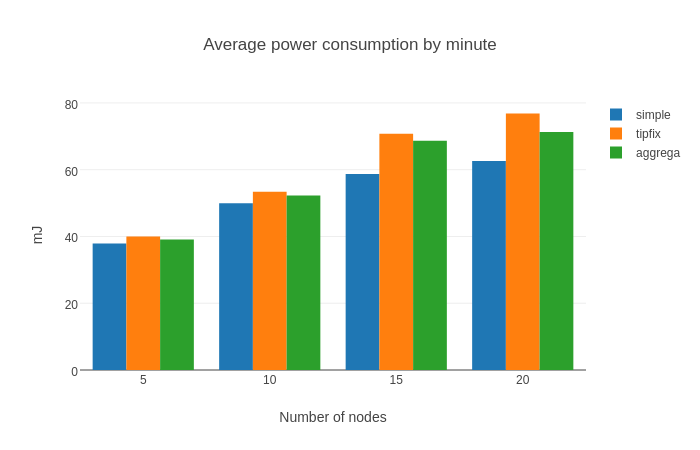
\includegraphics[width=\textwidth]{res/average_energy.png}
  \caption{Average energy consumption in mJ by minute}
  \label{fig:average_energy}
\end{figure}

From the chart we can conclude that by using aggregators inside the network we can reduce the added energy consumption induced by the usage of TinyIPFIX messages for monitoring purposes. As can be clearly seen when introducing more nodes, the energy consumption increases much more when not using aggregators. The graph on Fig.\ref{fig:increase_energy} shows exactly how the monitoring increase the energy consumption. The increase was computed by comparing the simple and aggrega configurations on their counterpart the simple configuration which do not send any information about the status of the network. As one may notice, the tipfix configuration consumes  relatively more energy when the number of nodes increases. However, it appears not to be the case with the aggrega one. Reasons may be due to the positions of the aggregators who impact greatly how the network behaves and thus weight on the power consumption. By placing intelligently the aggregators it is therefore possible to stress less the network.\\

\begin{figure}[h]
  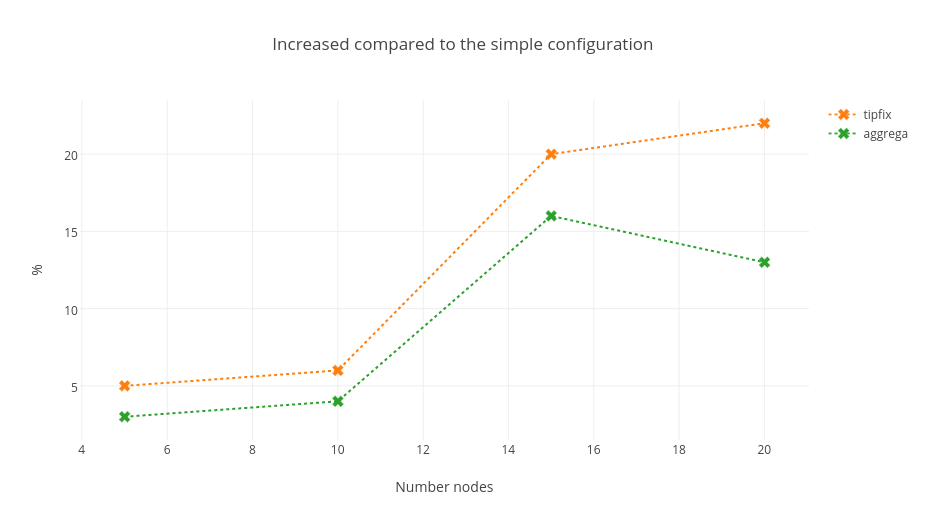
\includegraphics[width=\textwidth]{res/increase_energy.png}
  \caption{Increase in energy consumption induced by monitoring}
  \label{fig:increase_energy}
\end{figure}

\todo[inline]{explain why for 5 nodes exporters consume more}
One of the big advantage of also using aggregators is that it reduced drastically the load on the nodes that simply exports data and do not merge messages. This is depicted in Fig.\ref{fig:aggrega_energy}. The bar chart represents the energy consumption for the exporters and the aggregators in the aggrega configuration. Apart from the case with 5 number of nodes, all the case shows clearly that the exporters consume less energy than the aggregators with almost 20 mJ of difference for 15 nodes.\\

\begin{figure}[h]
  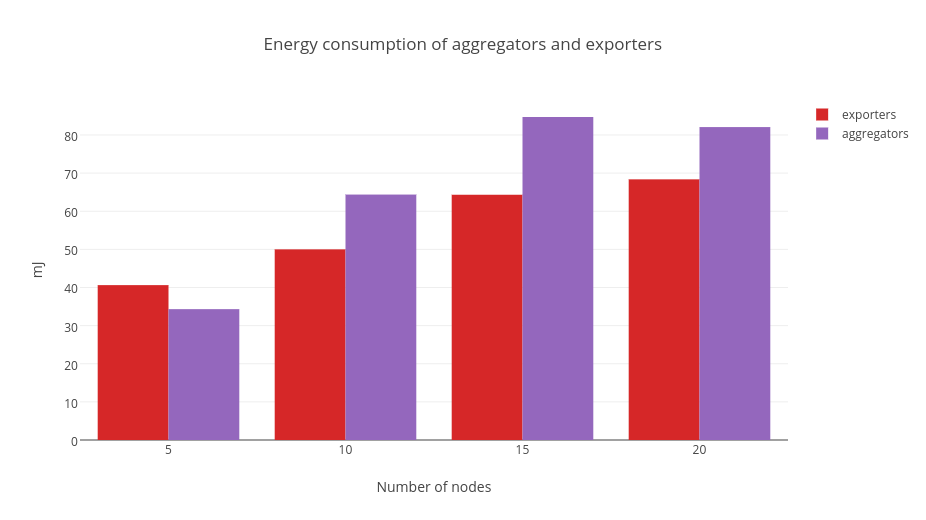
\includegraphics[width=\textwidth]{res/energy_aggrega}
  \caption{Energy consumption between aggregators and exporters}
  \label{fig:aggrega_energy}
\end{figure}

With those results, one may wonder how it affects the battery life of the nodes. The estimated lifetime of the battery is indicated in Tab.\ref{tab:battery_lifetime}. To compute those estimations we used the following formula

\begin{equation}
  lifetime = \frac{2400 mAh * 2}{X mW * 24 hours}
\end{equation}

where $X$ is the power consumption of a node. We used $2400mAh$ as we considered that the nodes were powered by AA battery. We multiply it by $2$ as the \textit{Zolertia Z1} uses 2 batteries. \\

The table shows clearly that to preserve the battery lifetime, aggregators become a must the more nodes are present in the IoT network.

\begin{table}
  \centering
  \begin{tabular}{|c|c|c|c|c|}
    \hline
    configuration & 5 nodes & 10 nodes & 15 nodes & 20 nodes \\
    \hline
    simple & 317 days & 240 days & 204 days & 190 days\\
    \hline
    tipfix & 300 days & 224 days & 168 days & 156 days\\
    \hline
    aggrega (exporters) & 294 days & 240 days & 186 days & 174 days \\
    \hline
  \end{tabular}
  \caption{Battery lifetime for different configurations}
  \label{tab:battery_lifetime}
\end{table}

\section{Nodes time repartition}

So as to more understand the power consumption induced by our solution, there is a need to see how often the nodes are active, and when it is the case what are they doing. To do so, we kept track on the time the nodes spend with their microprocessor active or in low power mode but also the time they were transmitting or receiving data via radio. This is what Fig.\ref{fig:time_all} shows. The Fig.\ref{fig:cpu_time} shows the average time the microprocessor is active by minute while Fig.\ref{fig:lpm_time} shows the average time the microprocessor is in low power mode. Fig.\ref{fig:tx_time} and Fig.\ref{fig:rx_time} shows average transmission time and receiving time by minute for a node. \\

\begin{figure}[h]
    \centering
    \begin{subfigure}[b]{0.45\textwidth}
        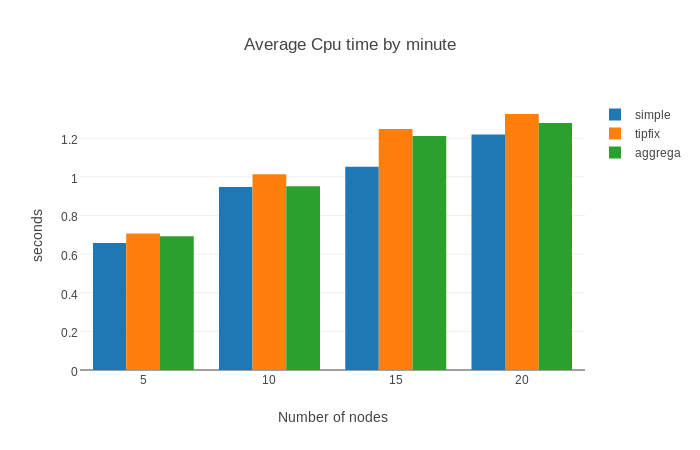
\includegraphics[width=\textwidth]{res/average_cpu}
        \caption{Average time spent with CPU active}
        \label{fig:cpu_time}
    \end{subfigure}
    ~
    \begin{subfigure}[b]{0.45\textwidth}
        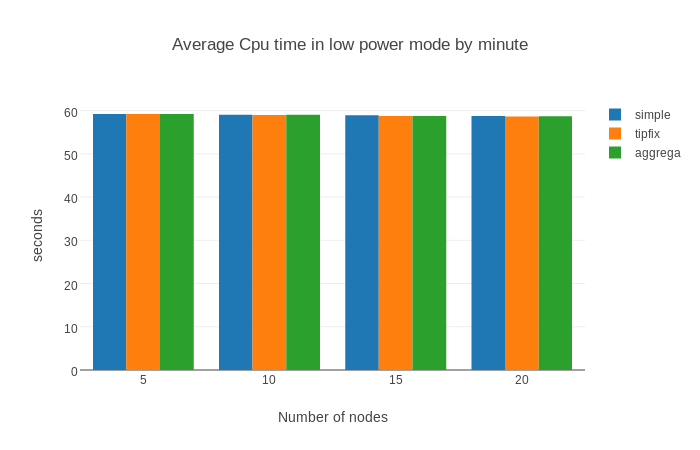
\includegraphics[width=\textwidth]{res/average_lpm}
        \caption{Average time spent with CPU in low power mode}
        \label{fig:lpm_time}
    \end{subfigure}
    ~
    \begin{subfigure}[b]{0.45\textwidth}
        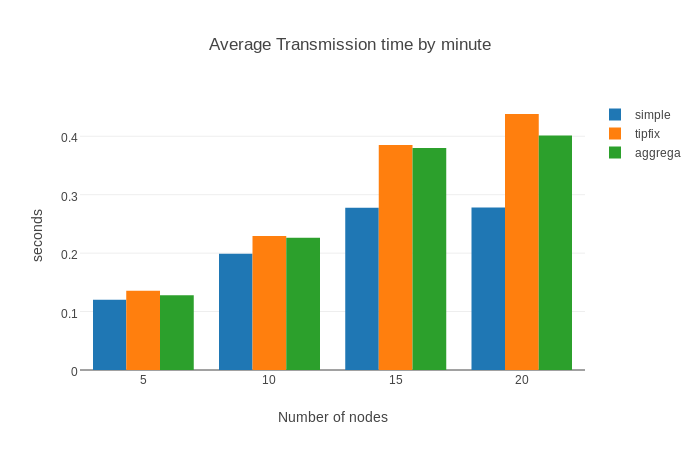
\includegraphics[width=\textwidth]{res/average_tx}
        \caption{Average time spent in transmission mode}
        \label{fig:tx_time}
    \end{subfigure}
    ~
    \begin{subfigure}[b]{0.45\textwidth}
        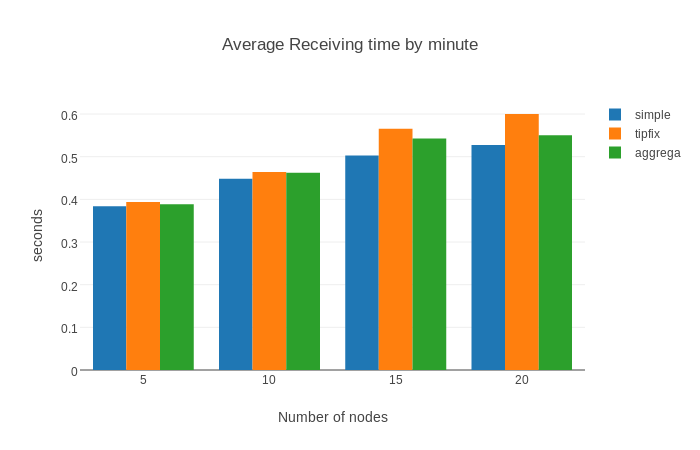
\includegraphics[width=\textwidth]{res/average_rx}
        \caption{Average time spent in receiving mode}
        \label{fig:rx_time}
    \end{subfigure}
    \caption{Average components time of nodes}
    \label{fig:time_all}
\end{figure}

The differences between the three configurations is highly visible for the transmission time and receiving time. In Fig.\ref{fig:tx_time} who shows the transmission time, we can clearly see than by monitoring, nodes pass more time transmitting data which influence the receiving time of the nodes. On Fig.\ref{fig:rx_time}, who shows receiving time, we can see that nodes receive more data which needs to be routed. It is however in the transmission time than there is the most gap between the configurations without and with TinyIPFIX.\\

However when analyzing the time spent with the CPU active on Fig.\ref{fig:cpu_time}, we can only notice than there is only a marginal difference between configurations with and without TinyIPFIX. This is also seen of Fig.\ref{fig:lpm_time} that shows the time the CPU is in low power mode. We can only conclude than the differential of energy consumption lies in the radio usage of the nodes induced by the sending of monitoring data. Increasing the interval at which nodes send their data could be a solution for network imposing as requirement a high battery lifespan.\\

We must emphasize the fact that using aggregators reduced the average time spent by the nodes transmitting or receiving but also with CPU active or in low power mode. The fact that TinyIPFIX messages are concentrated into one aggregator that merge them into one packets save the overhead caused by multiple headers from TinyIPFIX itself but also 6lowPan.


\bookmarksetup{startatroot}
\chapter*{Conclusion}
\addcontentsline{toc}{chapter}{Conclusion}

The Internet of Things presents many advantages that can bring a lot of positive things. Indeed, the IoT allows offers a lot of automation and thus avoid human intervention in specific situations, as well as optimizing energy consumption. However, the IoT presents a few challenges that explain why it has yet to be used more regularly. (peaufiner)\\

The subject of our thesis was to develop a monitoring tool of Internet of Things networks, using netflow on IoT devices to collect data about the current state of a network under analysis.\\

We have divided our thesis in three main parts.\\

In the first part, we have introduced \textit{the state of the art} of the Internet of Things. We have explained what it is, and what the smart objects composing such networks are. We have also discussed about its existing challenges that are the reasons why it is not widely deployed yet. We have also introduced the operating systems that are used in the IoT context, and why we have chosen Contiki as the main operating system. Part of the reason is due to the simulation software Cooja. To conclude the state of the art, we have introduced existing tools and technologies for the Internet of Things and also traditional networks. We have also specifically introduced Netflow (particularly IPFIX) and its principles, as it was among the technologies that were key to being able to monitor IoT networks and retrieve information about them. Additionally, we have introduced several existing monitoring tools that have been developed for traditional networks and IoT networks, and where the main differences with our own monitoring tool lie. One main difference is that the tools presented have set their sight on monitoring the sensors values while we wanted to focus on network traffic informations.\\

The second part describes our solution and how it responds to the problem of the thesis. It is divided into two chapters, chapters 4 and 5, one that explains the implementation of our software as the solution, the other one that showcases our software and explains how to use it.\\

More specifically, we have described in chapter 4 the whole architecture of our monitoring software. As explained, the architecture is divided in two subdivisions, one that is responsible for collecting data in a netflow fashion and sending it using TinyIPFIX messages, TinyIPFIX being a lightweight version of IPFIX (or Netflow v10). The TinyIPFIX messages are then reformatted into IPFIX messages by the gateway, and are then ready to be sent to the server. The second part of our archictecture is responsible for receiving and processing the collected information. The data is received from the gateway node of the IoT network to the server via UDP. Once the data is received, the server stores the messages in a database so that it can retrieve and process them. It also plays the role of a web server so as to present graphically the values stored in those messages. \\

We have also presented the technologies that we have chosen to use to develop our software and the reasons behind these choices. Indeed, we have chosen to use the technology Node.js that is quite convenient for developing HTTP servers, which is what we needed to develop a monitoring web-server. We also used the Express framework on top of Node.js. We found it convenient to develop a web-server as a software thanks to the ease with which one can install it along with accessing it, as it scales better with the number users having to use it at the same time. With the help of Javascript, we had an event-driven language, convenient for reacting promptly when the server IPFIX messages from the gateway node. Javascript also couples well with the JSON format that is convenient for dynamic websites such as ours. Along with using HTML and CSS for the visualization aspects of our software, we have used PostgreSQL as the database language for storing logs of data collected beforehand. Following the justification of our choices, we have described why our software is composed of four modules, the collector, the log, the Nodes Status, and the Web. Splitting the software into modules brings \textit{modularity} to the sotware, that can be further extended afterwards.\\

In chapter 5, we have written a guide on how to use the software and the different existing features, and depicted screenshots of it. As stated earlier, it is a web interface. There are two main tabs, one showing \textit{traffic volume} evolution through time, the other one showing a \textit{topology chart}. \\

The traffic tab contains several panels, all giving specific information about traffic volume generated in the network according to time, with specific filters such as IPFIX traffic, TinyIPFIX traffic, or normal traffic (regular packets sent between nodes). This tab also depicts specific statistics such as minimum and maximum bytes generated in a five-minutes interval and more generally some information about the network. \\

The topology tab showcases the current topology of the IoT network. The topology is an acyclic graph, more specifically a tree. All nodes composing the topology are clickable to obtain more specific information, such as its ID, its battery level, etc.\\

The third and final part was focused on the analyze of our solution. Mainly, the analyze was focused by the cost induced by the fact that nodes send meta information about the networks (the different flows). We clearly expressed this cost in term of energy consumption as one of the goal set for this thesis was to not excessively use the battery. To do so we used three different configurations depending on if the nodes send data for monitoring purposes by TinyIPFIX or had aggregators merging those TinyIPFIX packets. The results that came out were in favor of using aggregators so as to reduce the battery consumption. Also with 20 nodes, the estimated battery lifetime of nodes were reduced from 190 days to 174 days for exporters from a network using aggregators. A huge factor in the energy consumption was the radio usage time. Indeed, nodes sending TinyIPFIX packets spend more time transmitting and receiving data via radio which is quite logical.\\

Finally, this part also discusses about alternatives and possible extensions, as well as security. In this chapter, we discuss about Nfsen, a graphical web-based tool that provides a lot of monitoring information on IoT networks, using Nfdump. Nfsen was along with Nfdump the first technology that we started to work on to develop our monitoring software. However, as we have explained, we decided to use Node.js instead of Nfsen for conviniency and because it being more appropriate for the information that we wanted to retrieve from IoT networks and monitor. \\

We have also discussed about possible extensions to our software such as adding information about loads passing through links, handling network failures, and depicting protocol information on specific protocols such as UDP and RPL. We have also discussed about problems regarding security and what are the impacts of not taking security measures while monitoring the network which, in the current design of our software, is sensible to data tampering. Moreover, data is sent in the clear which would permit anyone to easily listen to the various communications.\\

In the end, those extensions have not been implemented because of them not being among the main purposes of our research. Most of the extensions require some change in the Netflow structure that we use to collect the data about flows, and require that motes have more capacities such as sending specific packets or being able to handle more situations.\\


\newpage

\nocite{*}
\bibliographystyle{amsplain}
\bibliography{biblio}

% Back cover page
\backcoverpage

\end{document}
